% class options:
% - select either [german] or [english]
% - select the type of thesis from:
%   [bachelor, master, generic]
%   (in case of generic, use \type{} to specify it)
% - use option "alpha" for abbreviated citation (instead of numbers)
% - option "draft" is available, too
% - use options "utf8" or "latin1" to select inputencoding
\documentclass[english, master, utf8]{base/thesis_KBS}

\usepackage[toc,page]{appendix}
\usepackage{units}    % useful for settings units:              \unit[23]{m}
\usepackage{nicefrac} % for setting fractions esp. within text: \nicefrac{km}{h}
\usepackage{subcaption}
\captionsetup{compatibility=false}

\usepackage{algorithm, algorithmic}  % for pseudo code (cf. documentation)
\renewcommand{\algorithmiccomment}[1]{\qquad{\small // \textit{#1}}}

% for code keywords within the text
\usepackage{xcolor}
\definecolor{light-gray}{gray}{0.95}
\newcommand{\code}[1]{\colorbox{light-gray}{\texttt{#1}}}

%%%%%%%%%%%%%%%%%%%%%%%%%%%%%%%%%%%%%%%%%%%%%%%%%%%%%%%%%%%%%%%%%%%%%%%%%%%%%%%

\begin{document}

\title{Execution Monitoring for Long-Term Autonomous Plant Observation with a Mobile Robot}
\author{Tim Bohne}
\email{tbohne@uni-osnabrueck.de}
\firstSupervisor{Prof. Dr. Joachim Hertzberg}
\secondSupervisor{Benjamin Kisliuk, M.Sc.}
%\shorttitle{...}                       % by default = title
%\dept{...}                             % by default KBS UOS
%\submitdate{November 2004}             % by default current month & year
%\signcity{}                            % by default Osnabr�ck
%signline{Osnabr�ck, 11. Dezember 2004} % by default "signcity, submitdate"

\generatetitle

\cleardoublepage

\begin{prefacesection}{Abstract}
TBD. \dots
\end{prefacesection}

\cleardoublepage
\tableofcontents

\startTextChapters %%%%%%%%%%%%%%%%%%%%%%%%%%%%%%

\chapter{Introduction}

ADD INTRO TEXT: Why is LTA interesting and relevant for agriculture?\newline

As the title suggests, the goal of this work is to integrate a prototypical system for long-term autonomous plant observation that is able to address 
particular challenges for long-term autonomy in such a context through the use of execution monitoring methods. Initially, typical challenges that may stand in the way of a mobile
robot's long-term autonomy in an agricultural setting will be identified. Afterwards, a subset of these challenges will be studied systematically in order to 
approach robust solutions. Accordingly, the prolonged objective is to increase the number of situations in which a mobile robot is able to 
overcome such challenges by itself. However, the mere recognition of problematic situations is already of decisive advantage from a practical perspective,
as the robot is then able to communicate the problem and request help, e.g. from a human operator, instead of undeliberately aborting its mission.
In addition, a prerequisite for solving a problem is, of course, recognizing it. Therefore, a major aim of this work is to develop execution monitoring
approaches that enable the robot to detect unexpected problematic situations that require special treatment.\newline

\textbf{Expected Scientific Contribution}\newline

Key challenges that may prevent long-term autonomous mobile robots in a field monitoring context from working properly will be identified, implemented 
in a simulation and systematically evaluated. A major objective of this work is to address a subset of these challenges based on execution monitoring approaches,
i.e. to propose methods that are capable of partially resolving or at least detecting such issues in order to enable the robot to communicate them to a human operator,
e.g. by a push message to the phone. The mere recognition of such situations would already be a decisive advantage from a practical perspective. Moreover, if it is possible
to show that with the solutions developed in this work the number of failures can be reduced by a certain percentage, distributed over a fraction of cases in which the robot 
recognizes a problem and calls the operator for help, and a fraction in which it is even able to solve the problem itself, the system can be considered a relevant step towards 
the overall goal of robust, long-term autonomous field monitoring robots. In other words, it is a suitable performance criterion that allows an empirical analysis to
determine whether the proposed methods are indeed able to improve the robustness of the system. In summary, this work attempts to reduce the barriers towards long-term
autonomy of mobile field monitoring robots by demonstrating a fully integrated solution capable of addressing some of the typical problems for such systems.\newline

\textbf{Approach}\newline

The idea is to start with the basic long-term autonomy setup described in section \ref{sec:prototype_scenario}, provide a list of potential problems that 
stand in its way, and develop execution monitoring methods to detect a subset of these issues with the aim of increasing the robustness of such a system in a simulation
and ideally in practice on the real hardware. In the end, there should be a working system that addresses some of the problems of long-term autonomy 
in scenarios similar to the one described in section \ref{sec:lta_plant_observation}. The nature of the work is going to be integrative and application-oriented. The modules 
needed to set up the initial prototype are available in principle, but it will be part of this work to integrate and extend them in order to end up with a holistic and robust
solution. After the basic scenario works in the simulation, it is going to be extended with an evaluation part. A subset of the potential barriers described in section 
\ref{sec:challenges_for_lta} is going to be implemented and it will be shown that the system no longer works under certain conditions, i.e. that these
barriers are indeed able to cause failure of long-term autonomous systems. Consequently, a first step is to observe how the system performs without any further 
treatment of such problematic situations, i.e. how often the robot gets stuck in the simulation based on a specific problem case.
Subsequently, the goal is to develop monitoring methods capable of recognizing these problems such that they can be resolved.
To give an example, a particular idea could be to block paths on the field in the simulation in a randomized fashion with the intent of reproducibly making things that 
can go wrong actually go wrong. The type of the obstacles is incidental to this work, e.g. a muddy path that the robot is not able to drive through. 
It is obvious that the robot must be enabled to detect such problems, in this case by some kind of obstacle detection.
Once detected, the problem can be resolved by either incorporating solutions from the literature or finding new solutions.
Since detection is a necessary prerequisite for overcoming these barriers, the focus will be on detection, i.e. execution monitoring,
and an initial trivial solution adopted for all of them is to call the human operator who then takes care of the problem.\newline
As should be clear by now, long-term autonomy, as robotics in general, is an integration problem. Many technologies have to be integrated in order to build a working system, 
and compared to other disciplines of artificial intelligence, it is not trivial to evaluate the system and conclude, for example, that it has improved the status quo by a 
certain percentage. Nevertheless, it is crucial to provide results that are meaningful based on scientific standards. 
The keyword under which such attempts are summarized is scientific robotics, and a goal of this work will be to evaluate the developed system based on these standards.
Since it is beyond the scope of this work to test the developed system for extended periods of time in practice, there is a need for other ways of evaluation.
This is where the described evaluation approach in the simulation comes into play. In order to demonstrate, test and evaluate the system, there will be a sufficiently meaningful, 
i.e. realistic, physics simulation that allows an empirical analysis based on a huge number of samples. As mentioned, the starting point will be the simulation from the 
PORTAL project that is going to be extended as part of this work. Ultimately, there should also be a long-term test (e.g. one day) in the field with the real hardware that 
underlines the relevance of the approaches discussed in this work for practical applications. However, since a mobile robot is a complex system, there are arbitrary 
many technical barriers that could prevent such a long-term test in the real world. The idea is therefore to be at least able to demonstrate the system in the simulation
without depending on the success of such a real-world experiment. In addition to serving as a backup for possible failures in real-world tests,
a simulation naturally creates an environment that allows reproducible situations and thus permits empirical investigation.

ADD CHAPTER OVERVIEW \dots\newline

\chapter{Long-Term Autonomous Mobile Robots}

Long-term autonomous mobile robotic systems can be of great benefit in diverse environments. For the most part, in activities that are either too dangerous,
or too undemanding (e.g. monotonous, not meaningful) to be performed by humans. In addition, economic considerations can play a role, as well as tasks 
that are undesirable for other reasons, e.g. because they are considered dirty.
All three attributes - \textit{long-term}, \textit{autonomous}, and \textit{mobile} - have the potential of dramatically increasing the complexity and
the risk for failures of the system. Part of this chapter will be to precisely define what each of the attributes means in the context of this work.
The attribute of mobility is the easiest to define: A mobile robot is a system capable of moving freely (within limits) through an environment. \cite{Hertzberg:2012}
Thus, it's about the ability of a robot to move rather than being statically attached to a position.
Section \ref{sec:lta_plant_observation} introduces the scenario that is going to be studied in this work and provides a definition for the concept of long-term 
autonomy as understood in the following chapters, i.e. clarifies what the two remaining attributes \textit{long-term} and \textit{autonomous} are supposed to mean.
Afterwards, in section \ref{sec:scientific_bg}, the scientific and technological background that forms the basis of this work is discussed. 
Finally, section \ref{sec:challenges_for_lta} identifies potential hinderances for long-term autonomous systems with a particular focus on the considered plant monitoring scenario.
TODO: update..\newline

\section{Literature Review - State of the Art}
\label{sec:literature_review}

Kunze et al. point out that many challenges remain to be overcome with respect to the reliable deployment of long-term autonomous robots in real-world environments.
Particularly relevant to this work are the natural challenge of system integration, i.e. integrating numerous methods and technologies into a comprehensive solution 
for long-term autonomy, as well as the design of ``human-in-the-loop'' systems capable of utilizing the help of human operators in unexpected problematic situations. \cite{Kunze:2018}

\section{Long-Term Autonomous Plant Observation}
\label{sec:lta_plant_observation}

The particular scenario that is going to be considered in this work takes place in an agricultural context.
The idea is to enable a mobile robot to autonomously conduct 3D-Lidar scans and hyperspectral images of the plants on a field in order to monitor their growth progression and 
to detect certain features based on the growth stage. Moreover, these recordings can be used to detect leaf diseases [TODO: refine based on literature].
Correspondingly, the robot has to be able to process the entire field continually without the need for human supervision,
including the requirement for repeated charge stops. For this purpose, there is supporting infrastructure in the form of a container with an inductive charging station on site
establishing the power supply. Since the focus of the work is not going to be the scanning task, but to establish robust long-term autonomy, the actual detection of features 
etc. will be disregarded.
A crucial question is how to actually define ``long-term''. As Hawes et al. remark, it has no strict definition and can have various meanings depending
on the context, e.g. NASA's rover \textit{Opportunity} has been exploring the surface of Mars autonomously for years and autonomous wave gliders are able to monitor
ocean sections for months. Furthermore, there are mobile service robots used for extended periods of time in everyday, indoor environments like hospitals 
as examined in the STRANDS project. \cite{Hawes:2017}
For this work, in contrast, ``long-term'' is going to be defined in terms of the robot's temporal radius of action that is mainly based on its battery capacity, i.e. charge cycle,
but may also include aspects like maintenance intervals etc. In general, all processes that require a number of such cycles are considered long-term processes.
Accordingly, ``long-term'' can only be defined depending on the system in question. To give an example: There are systems with very limited battery capacity, 
such as toy drones. Based on absolute time, a two-hour experiment might not be regarded as being long-term, but if it involves multiple charging cycles, it can be 
algorithmically considered a long-term process. Consequently, ``long-term'' is relative.\newline
In the agricultural sector, there are processes that last much longer than a charge cycle, e.g. vegetation periods.
However, the seasonal cycle is not the sort of long-term process that will be investigated in this work, as such processes already exist on a much smaller scale.
On the one hand, there is the mission level, i.e. one processing of an entire field. 
Such a mission can already be regarded as long-term, since based on the dimensions of the particular field under consideration, it is not guaranteed that one
battery charge will be sufficient to process the entire field. Instead, one battery cycle will be defined as sufficient to process a certain fraction of the scan
positions, and a planner should maximize the number of planned scan stops in a mission under the constraint that a battery safety buffer is not undercut.
Thus, a key aspect of the scenario is going to be that the mission must be paused, the state must be saved, and the mission must be continued after recharging.
In the meantime, the environment may have changed, e.g. weather conditions or illumination, which is relevant for certain sensors of the robot.
On the other hand, there are going to be several such field processings during one vegetation period, which makes it a long-term process of repeated missions.
Hence, it takes a number of charge cycles to process the entire field, and that mission is going to be repeated every few days,
which means that there are two different long-term cycles that are intertwined.
These two cycles basically represent a lower bound for the length of long-term autonomous episodes in the scenario under
consideration. Likewise, in contrast to the above examples of Mars rovers and autonomous wave gliders, which are long-term
processes of arbitrary length, it is useful to think about natural upper bounds on the length of such episodes in agricultural
applications. Such a natural upper bound could be a time after which a human operator will inspect the robot anyway,
which in agriculture is certainly the case sooner than after a few months, e.g. during maintenance sessions 
when sensors such as cameras and laser scanners are cleaned, tire pressures are checked, etc.
After such a maintenance session, the new episode begins. 
Based on these bounds, it makes sense that the robot does not send every minor problem it recognizes directly to the operator,
but keeps a list of minor issues that do not require immediate action, but should be resolved during the next maintenance
appointment.\newline
Now that it has been sufficiently clarified how \textit{long-term} and \textit{mobile} are to be understood in the context of this work,
a precise definition of what is meant by the remaining attribute \textit{autonomous} follows.
Like the concept \textit{long-term}, \textit{autonomous} is not sharply defined in the literature and can have different meaningful connotations depending
on the context. Autonomy in the context of application-oriented robots usually has the goal of achieving a higher degree of automation in these applications,
i.e. using technical means so that a process runs completely or partially without involvement and supervision of a human operator. \cite{Hertzberg:2015}
Completely or partially already indicates that autonomy is not a binary attribute, but refers to a spectrum of different degrees of autonomy,
ranging from teleoperation at the lower end over shared and traded control up to full autonomy at the upper end. \cite{Hertzberg:2015}
Figure \ref{fig:autonomy_spectrum} summarizes these concepts based on \cite{Hertzberg:2015}.
\begin{figure}[H]
    \centering
    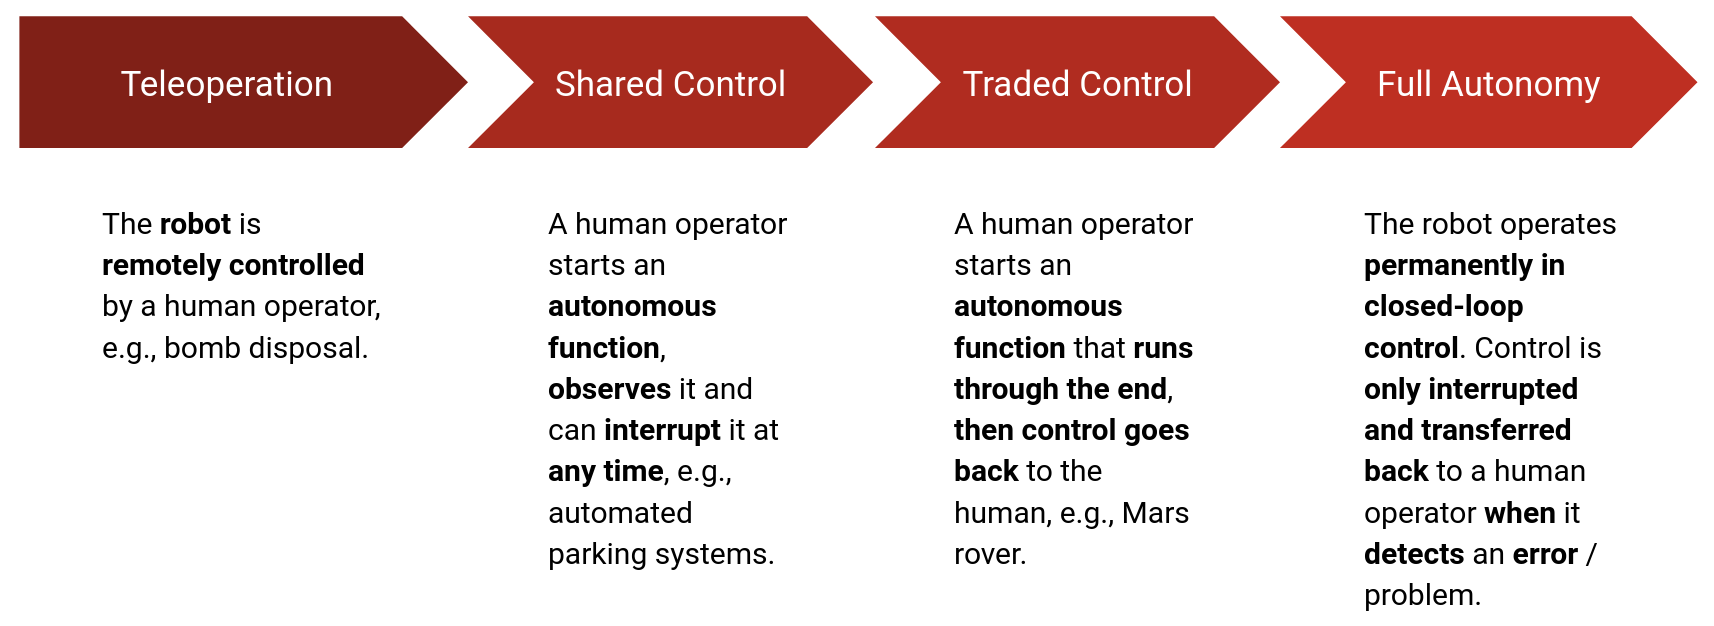
\includegraphics[width=\textwidth]{pics/autonomy_spectrum.png}
    \caption{\textsc{Autonomy Spectrum}}
    \label{fig:autonomy_spectrum}
\end{figure}
\noindent
Accordingly, autonomy does not necessarily mean that there is no connection to a human operator at all.
The concept of traded control is particularly relevant for robotics in space applications, e.g. satellites or planetary rovers.
The idea is that the robotic system operates autonomously in principle, performing all the repetitive routine tasks, but the human operator can take over in certain situations,
such as when the robot is in danger and human intervention is required, or when a task needs to be performed that for some reason is better suited for a human operator.
\cite{Kortenkamp:2009}
The plant monitoring robot considered in this work, however, can be classified as fully autonomous in the sense of figure \ref{fig:autonomy_spectrum}, 
i.e. during a long-term autonomy cycle as defined above, the robot should only come into contact with a human operator when it detects an error or a problematic situation
that prevents it from continuing its task.

\section{Robotic System and Infrastructure}
\label{sec:robotic_system}

The robotic system under consideration is going to be the autonomous robotic experimentation platform (AROX) \cite{Kisliuk:2021} that is depicted in figure \ref{fig:arox_system}.
It is assumed to integrate all the essential software and hardware required for the task at hand, i.e. processing a given plan (e.g. human provided) that causes the robot
to autonomously drive to specified locations and record scans. As discussed, this should be possible over extended periods of time, i.e. long term, including charge stops, etc.
According to Kunze et al. \cite{Kunze:2018}, different areas of AI must be brought together to enable long-term autonomous robots in practical applications.
As essential building blocks, they identify \textit{navigation \& mapping}, \textit{perception}, \textit{knowledge representation \& reasoning}, \textit{planning},
\textit{interaction}, and \textit{learning}. All of these aspects will be part of the following description of the AROX system, except \textit{learning}, for which, however, 
useful applications have already been identified that could improve the long-term autonomy performance of the system in the future.\newline
The AROX consists of a two-axle (2WD differential drive) mobile platform based on an \textit{Innok Heros}\footnote{https://www.innok-robotics.de/produkte/heros}. \cite{Kisliuk:2021}
In addition to the AROX system itself, Kisliuk et al. introduce a supporting infrastructure in the form of a mobile base station (container) at the field site,
which provides an inductive charging station, a mobile internet connection and a WiFi network for local data exchange.
Real-time kinematics (RTK) is used, a differential GNSS\footnote{Global Navigation Satellite System} method that results in high-precision positioning (in centimeter range)
near a base station, such as the mobile container. The errors or inaccuracies of basic GNSS techniques are avoided in RTK solutions by transmitting correction signals based
on carrier measurements of the base station, whose location is precisely known. \cite{RTK_fundamentals} For this purpose, the container also provides an NTRIP server.
Besides these technical features of the container, it also simply serves as a shelter for the robot.
In order to actually use RTK, a real-time communication channel (e.g. WiFi) is needed to connect the RTK base station, i.e. the mobile container, with the RTK rover,
i.e. the AROX, to transmit the aforementioned correction signals. Furthermore, it is crucial that both the robot and the base station receive their own GNSS signals, 
i.e. are connected to the GNSS service. The AROX also maintains WiFi or LTE connections for the purpose of transmitting the recorded scans to external servers or the base station.
The robot's localization is multi-layered and based on sensor fusion of IMU, odometry and RTK-GNSS data using the \code{robot\_localization} \cite{Moore:2014} package.
Several laser scanners are attached to its base and used to avoid collisions, e.g. the \textit{SICK TiM} and the \textit{Velodyne Puck} mounted at the optional sensor
slots displayed in fig. \ref{fig:arox_system}. For the actual task of plant monitoring, the high-resolution 3D-Lidar sensor \textit{RIEGL VZ-$400$i} is used,
which can be combined with a calibrated hyperspectral or RGB camera (cf. fig. \ref{fig:arox_system}). \cite{Kisliuk:2021}
For navigation, the ROS package \code{move\_base\_flex} \cite{Puetz:2018} is used, a more flexible extension of the standard ROS navigation framework \code{move\_base}.
The primarily used path planning algorithms are provided by the ROS packages \code{eband\_local\_planner} and \code{dwa\_local\_planner}.
In addition to the actual physically available AROX, the system has been modeled in the unified robot description format (URDF) and can be used in a simulation.
\begin{figure}[H]
    \centering
    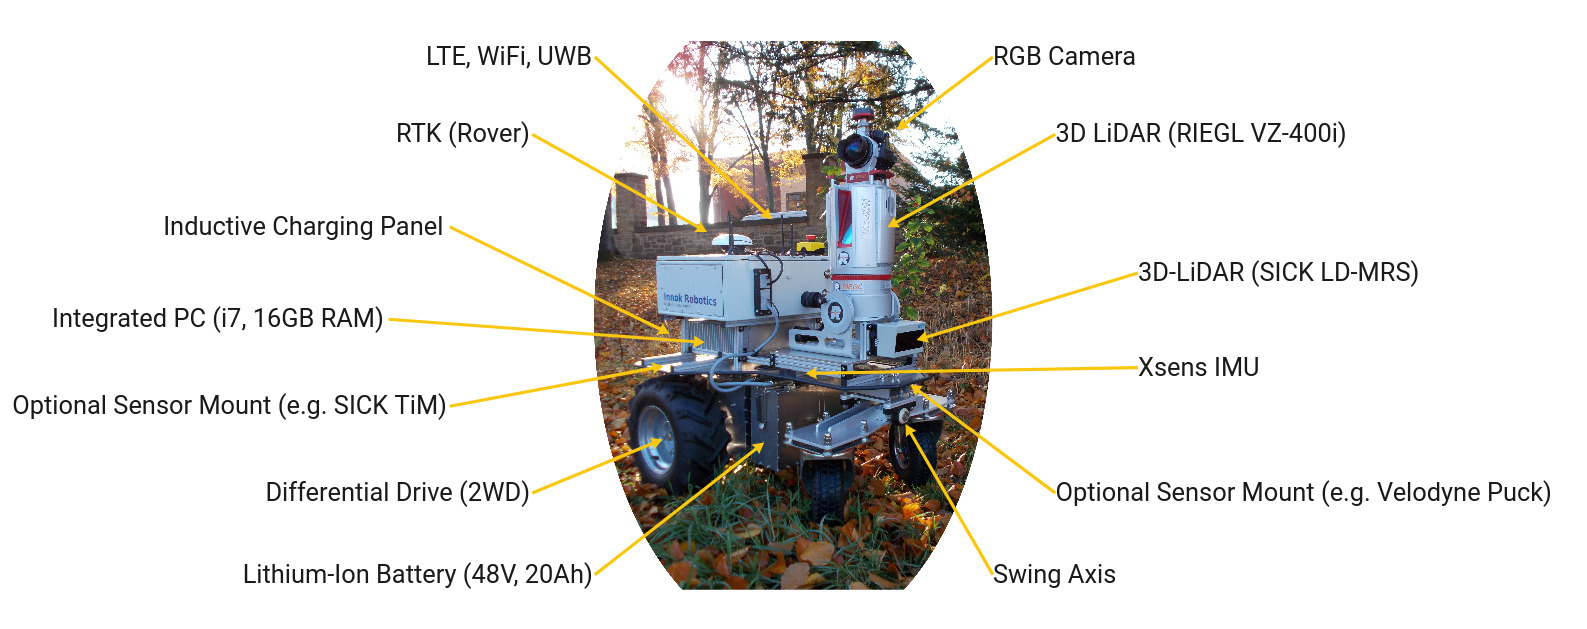
\includegraphics[width=\textwidth]{pics/AROX.jpg}
    \caption{\textsc{Autonomous Robotic Experimentation Platform (AROX)}}
    \label{fig:arox_system}
\end{figure}

\pagebreak

\section{Prototype Scenario in the Simulation}
\label{sec:prototype_scenario}

As starting point serves a physics simulation in Gazebo\footnote{Open-source 3D robotics simulator} that has been created within the research project PORTAL \cite{portal}
and is adapted and extended as part of this work. The simulation includes the AROX model, i.e. a simulated version of the system described in section \ref{sec:robotic_system},
as well as a 2.5D reflection of a test field environment. For the prototypical baseline scenario of this work, the layout of abstract crops as objects of interest shown in 
figure \ref{fig:prototypical_layout} was created. Initially, the simulation works under the assumption that the robot is able to charge its battery as soon as it is located at 
certain coordinates as a simplification of the container infrastructure. These coordinates are visualized by the charge patch displayed in figure \ref{fig:prototypical_layout}.
In order to determine the robot's route through the field as well as the whole scanning processes, a plan is needed, i.e. when to drive to and process which parcel of the field. 
An example of a simple scan route can be seen in figure \ref{fig:example_scan_route}. Since this work does not deal with planning algorithms, it is simply assumed that the plans
are created by human operators. Hence, a plan is going to be a CSV file of actions. Plan generation and format are described in detail in section \ref{sec:plan_generation}, 
but in general plans will focus on two types of actions. The first type is \code{drive\_to$(lat, lng, \theta)$}, which causes the robot to drive to the specified latitude, 
longitude, and orientation (if possible), an action the employed robotic system AROX is capable of. The second type of action is \code{scan}, which initiates a scanning procedure
at the robot's current position. In practice, the real robot is equipped with a high-resolution 3D-Lidar sensor (cf. RIEGL sensor in fig. \ref{fig:arox_system}) that is going 
to be used to scan the field parcels with the aim of detecting features of the plants. To simulate the scanning procedure, some kind of dummy node is required that allows to 
scan on command (cf. section \ref{sec:dummy_scanning_node}), i.e. to simulate scanning, since we are not actually interested in any real scanning data. Thus, the second type 
of action will initiate a scanning procedure of the 3D-Lidar sensor or an execution of a dummy node, respectively. There are other actions, but these two are the very specific ones
relevant to the scenario under consideration; the details are described in section \ref{sec:plan_generation}. This prototypical scenario is the implementation of a minimal 
example of a long-term autonomous plant monitoring scenario in a simulation. Basic autonomous long-term functionality is provided, which means that the robot is able to 
complete its plant observation missions interrupted by several necessary charge stops. It will be used later to evaluate the challenges identified in section 
\ref{sec:challenges_for_lta} as well as the monitoring approaches presented in section \ref{sec:monitoring_for_lta_challenges}.
The overall process implemented for each of the challenges considered is to simulate the occurrence of the respective issue, detect it using
the monitoring approaches developed in this work, interrupt the robot's normal operation, solve the problem, and transition back to normal operation to resume 
plan execution exactly where it was preempted.
\begin{figure}[H]
    \centering
    \begin{subfigure}[b]{0.49\textwidth}
        \centering
        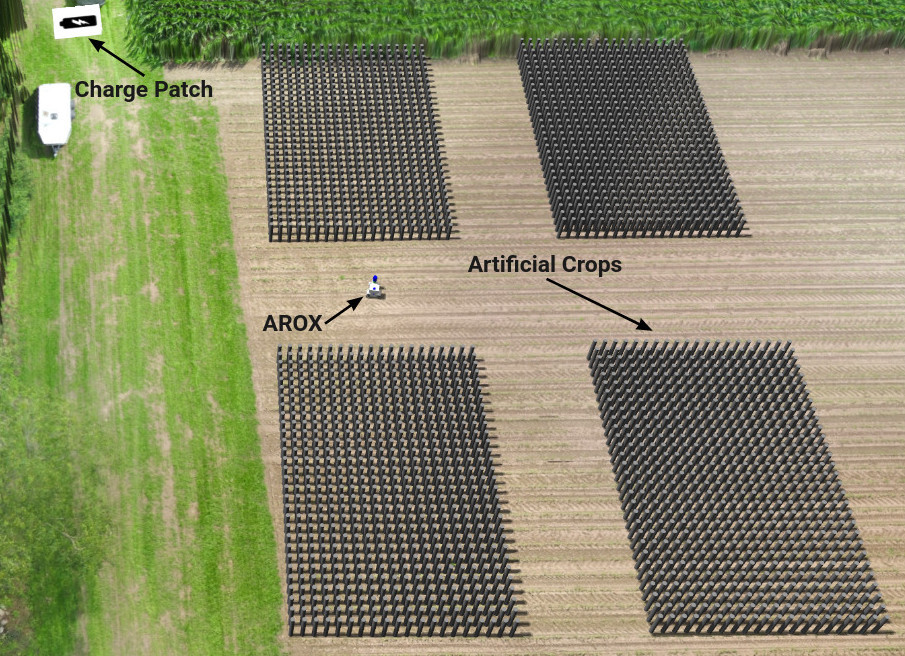
\includegraphics[width=\textwidth]{pics/prototype_scenario.jpg}
        \caption{\textsc{Prototypical Layout}}
        \label{fig:prototypical_layout}
    \end{subfigure}
    \hfill
    \begin{subfigure}[b]{0.49\textwidth}
        \centering
        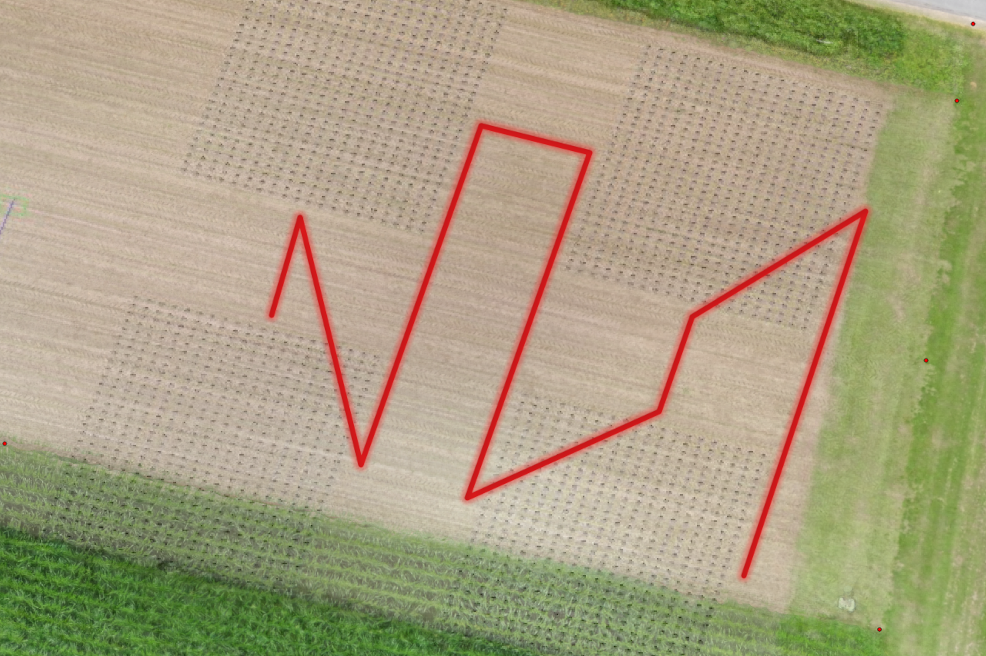
\includegraphics[width=\textwidth]{pics/example_path.png}
        \caption{\textsc{Example Scan Route}}
        \label{fig:example_scan_route}
    \end{subfigure}
\caption{\textsc{Prototype Scenario in the Simulation}}
\label{fig:prototype_sim}
\end{figure}

\subsection{Dummy Scanning Node}
\label{sec:dummy_scanning_node}

Since the scenario described in the previous section assumes a representation of a \code{scan} action, but the work does not really depend on realistic scan data,
a pragmatic solution is required. The result is a dummy node implementing a ROS \code{SimpleActionServer} that simulates the results of the \textit{RIEGL} scanner
(cf. fig. \ref{fig:arox_system}). It is expected that a \code{scan} action will trigger an incoming \code{LaserScan} on the topic \code{/RIEGL}, which will then be
written to a file to also have some form of data management. Since the \textit{Velodyne} LiDAR sensor is already part of the simulation and the nature of the incoming data
is essentially the same, a \code{scan} action just leads to one republished \textit{Velodyne} scan under the \code{/RIEGL} topic using \code{rospy.wait\_for\_message()},
which merely creates a subscription to the topic, receives one message, and then unsubscribes. The incoming data is basically a list of distance values for certain angle-height 
combinations along with arbitrary many metadata such as minimum angle, maximum angle, scanning time, and identifier. Thus, the dummy node enables the \textit{Velodyne} sensor
to briefly pretend to be a \textit{RIEGL} sensor. This approach has the useful side effect of making it relatively easy to simulate sensor failures by simply stopping to
republish the \textit{Velodyne} after a \code{scan} action (cf. section \ref{sec:simulation_of_lta_challenges}).\newline
The actual real \textit{RIEGL} sensor scans are of data type \code{PointCloud2}, and the monitoring solutions described in section \ref{sec:monitoring_for_lta_challenges}
are capable of processing incoming scans of types \code{LaserScan} as well as \code{PointCloud2}. It is configurable in which form the data should be received. The first
option is that the sensor makes the scans available to the ROS system via a topic, i.e. the sensor publishes the scans under a topic. These scans could potentially be reduced,
e.g. only every second value is published to reduce the overall size, because if the scans become too large, it is no longer viable. The second option is to specify a 
directory path and write the scans to the file system, where the scanner creates \code{.ply} files containing the scans in a human-readable ASCII format.
The two options result in the need for two different types of monitoring. If the scans are published to a specific topic, it is sensor monitoring.
If they are written to the file system, it is data management.

\pagebreak

\section{Challenges}
\label{sec:challenges_for_lta}

Having clarified what long-term autonomy (LTA) means for this work, we now turn to potential problems that stand in its way.
There are numerous potential hinderances for long-term autonomous systems that can cause failure and prevent the system from continuing its task.
The following three constraints precisely define the LTA problems considered in this work.
\begin{enumerate}
    \item It can practically occur in the concrete scenario described in section \ref{sec:lta_plant_observation}.
    \item It can prevent the smooth functioning of LTA systems or affect the quality of its results.
    \item It can be detected by monitoring methods and subsequently solved or communicated.
\end{enumerate}
This definition contains certain implicit assumptions. The first constraint, for example, implies that these problems should have some probability of occurring,
i.e. they should be relatively likely to occur. Accordingly, potential problems such as lightning strikes or wild boar attacks are ignored because they are highly 
unlikely and also difficult, if not impossible, to solve. Moreover, many of the issues of this rather unconventional type, if solvable, could in principle be covered
by more general classes of problems from the following list. Furthermore, the third constraint, i.e. that the considered problems can be detected and subsequently solved 
or communicated, assumes that the system is still fundamentally functioning and has not completely collapsed; a counterexample would again be a lightning strike.
Without claiming to be exhaustive, the following is a list of potential problems in an agricultural field monitoring context that, 
from a practical perspective, fulfill the above restrictions and are thus worthy of investigation:
\begin{itemize}
    \item \textbf{power management} (battery failure / unexpected low battery)
    \item \textbf{charging failure} (unsuccessful docking / no charging)
    \item \textbf{drastic weather change} (e.g. storm, fog, extreme sunshine, heavy rain, extreme cold)
    \item \textbf{certain dynamics} (e.g. day / night)
    \item \textbf{sensor (perception) failure}
    \item \textbf{perceptual aliasing issue}
    \item \textbf{data management} (e.g. full memory, sensor data processing failure)
    \item \textbf{lost connection} (WiFi, RTK, UWB, LTE)
    \item \textbf{obstacles blocking planned path} (static / dynamic)
    \item \textbf{robot gets stuck} (e.g. spinning wheels)
    \item \textbf{robot falls over}
    \item \textbf{navigation failure} (\code{move\_base\_flex} / \code{pdc})
    \item \textbf{sustained recovery}, i.e. no return to normal operation
    \item \textbf{incorrect / inaccurate localization} (GPS, IMU, odometry)
    \item \textbf{mapping error} (e.g. incorrect costmap entries)
    \item \textbf{plan deployment failure}, i.e. robot remains in idle state
\end{itemize}
For each potential problem identified, its relevance and consequences, i.e. a brief description of why it might be problematic, is provided below.\newline

\noindent
\textbf{Power Management}\newline

\noindent
A natural requirement for LTA systems as defined in section \ref{sec:lta_plant_observation} is some form of energy management.
The system is expected to operate autonomously for extended periods of time, which of course assumes a power supply. 
However, the energy management estimated at planning time may not work correctly or as expected at execution time, e.g. the battery could be 
low before the planned time. Or worse, there could be a complete battery failure. It would certainly be useful to enable the system to handle such issues, at least to 
some degree.\newline

\noindent
\textbf{Charging Failure}\newline

\noindent
Another category of potential LTA problems related to the system's power supply is charging failures. Several things can go wrong during a charging process. 
Leaving aside the simplistic assumption of charging upon arrival at specific coordinates and considering the actual charging process 
in practice with the AROX system, it must dock with an inductive charging station in a mobile container at the field site.
Accordingly, docking to the charging station may fail or the charging process itself may not start after docking.
Both cases lead to a failed charging process and thus to an abortion of the robot's LTA mission. An evaluation of potential docking failures would require 
integration of the autonomous docking / undocking solution described in section \ref{sec:docking_solution}.\newline

\noindent
\textbf{Drastic Weather Change}\newline

\noindent
Since the system is designed for moderate weather conditions, drastic weather changes can also play a role.
If the weather changes too drastically, it can be problematic for various aspects of the system.
If it is stormy, for example, this can be delicate for the sensor recordings, but also for the robot platform itself, as it could fall over.
The quality of the sensor images can also be affected by fog or extreme sunlight (illumination).
In addition, heavy rain should also be avoided. Finally, extreme cold could be a major problem for the system's battery.\newline

\noindent
\textbf{Certain Dynamics}\newline

\noindent
Similar to weather changes, there are other dynamics such as the natural transition from day to night. For sunlight-dependent sensors such as cameras, 
the robot should take twilight into account and plan its operations accordingly to be back in the shelter, i.e. the mobile container, by dark.\newline

\noindent
\textbf{Sensor (Perception) Failure}\newline

\noindent
Hardware issues are a very general problem class and could relate to almost arbitrary many kinds of problems. Since the correct functioning of the 3D-LiDAR sensor is
crucial for the long-term monitoring scenario described in section \ref{sec:lta_plant_observation}, the main focus will be on detecting hardware faults of this type. 
Sensor failures are, of course, a failure class in which the robot can do little except attempt to restart the corresponding sensor, and therefore rarely has any choice but to 
call the human operator for assistance. Nevertheless, it is important to identify such a malfunction as soon as possible, communicate the problem and avoid a lot of useless work 
and wasted operating time. Obviously, total sensor failures are realistic in practice for any LiDAR sensor, or even any sensor in general, due to a hardware fault, an interrupted
power supply, or a variety of other reasons. However, there are more subtle failures than just a total breakdown, and the incoming scan data should be checked for plausibility.
From a practical point of view, it is a valid assumption to receive the scans via a specific ROS topic. One issue could be an empty list of range values, i.e. a scan arrives on
some ROS topic but is essentially vacuous. As mentioned in section \ref{sec:dummy_scanning_node}, the crucial part of a laser scan is the list of range values, which makes it 
useless if this list is empty for some reason. Its realism could be debated, and of course it is pointless to detect problems that do not occur in practice. However, since it is
relatively easy to simulate and detect, it is treated as a basic test that can be used, for example, to detect problems due to implementation-specific errors.
Another, more subtle problem could be a scan that mainly contains values that do not satisfy the sensor's maximum or minimum range, i.e. \code{inf}, which may indicate that
the robot has fallen over, or the sensor has slipped out of position. This could indicate, for example, that the sensor is pointing towards the sky, causing the values to exceed
the maximum range. However, depending on the sensor used and the environment, in large open fields the nearest objects that could be detected may actually be farther away and exceed
the maximum range of the sensor. Analogously, the same problem occurs if an object is too close to the sensor, i.e. the minimum range is undercut. In both cases, the sensor only
returns \code{inf} values. It should be detected when the list of range values is predominantly filled with impermissible \code{inf} values. Finally, it could be a problem if the
same scan is published repeatedly. It is possible that the range values between two scans where the robot has not moved are similar, although they should never be the same due to
noise, etc. However, what should be different in each case is the metadata such as the ID.\newline

\noindent
\textbf{Perceptual Aliasing Issue}\newline

\noindent
Place recognition can certainly be useful for LTA operation of a mobile robot. However, long-term place recognition is not trivial because 
the appearance of places in the environment changes quite drastically over time, e.g. due to illumination, vegetation periods, or weather. \cite{Han:2018}
In the scenario considered in this work, it is particularly relevant that the robot is able to recognize the place of the mobile container
that serves as shelter and provides the charging station. In addition to the natural changes in the environment over time, there is another important aspect
that makes long-term place recognition particularly challenging - the perceptual aliasing issue. This problem refers to the fact that certain places and objects are very 
similar to each other, that is, they have many common characteristics, which makes them hard to distinguish. \cite{Han:2018}
If, for example, a mobile office container is placed right next to the robot's base station, it might be difficult for the robot to distinguish the objects.
Hence, there could be a need for monitoring methods that are capable of recognizing such situations and providing some strategies to resolve the perceptual aliasing issue.\newline

\noindent
\textbf{Data Management}\newline

\noindent
Since the overall objective of the robot's missions is to acquire data, the appropriate management of this data is of relevance.
If, for example, the robot is no longer able to save further scans due to a full memory, it should recognize and communicate this.
In addition, there may be disturbances in the processing of the sensor data, so that the robot is no longer able to process and save the recordings correctly.
Successful scanning is worthless if the resulting data is not saved properly, so it is important to monitor whether the scans are being written to a file correctly.
Therefore, tt would be valuable to identify such problems as soon as possible to avoid redundant missions.\newline

\noindent
\textbf{Lost Connection}\newline

\noindent
For the robot to work as expected, it must maintain connections to various services. Accordingly, an interruption of one of these connections should be detected immediately.
A real time communication channel (e.g. WiFi) is required to connect the RTK base station, i.e. the mobile container, and the RTK rover, i.e. the robot, in order to
transmit the correction signals for high-precision positioning. Furthermore, it is crucial that both the robot and the base station receive their own GNSS signals,
i.e. are connected to the GNSS service. In addition, the RTK-GNSS data is used for scan registration. Finally, the recorded scans are transmitted via WiFi or LTE 
to the base station or external servers for further processing.\newline

\noindent
\textbf{WiFi Connection Failures}\newline

\noindent
The most common form of WiFi failure, which is very relevant and realistic in practice, is of course a simple disconnection.
However, there are again more subtle problems than just the complete absence of a connection, so the quality of an established connection should also be monitored.
Generally, network monitoring can be done arbitrarily detailed, for this work it is limited to some attributes that allow a general statement about the quality of
the connection in practice. One realistic problem is an overall poor link quality, which is a measure combining different kinds of metrics, e.g.
\textit{Received Signal Strength Indication} (RSSI), \textit{Signal to Interference plus Noise Ratio} (SINR), \textit{Packet Delivery Ratio} (PDR), and
\textit{Bit Error Rate} (BER). \cite{Vlavianos:2008} Another well-known problem with WiFi systems is a poor signal, i.e. a low RSSI value. The RSSI is already part of
the link quality assessment, but due to its practical importance, it is also worth to be considered in isolation. Furthermore, the bit rate, i.e. the speed at which
information is transmitted, gives a good indication of the overall connection quality, and it should be recognized when it falls below a certain threshold, which is a
lower limit for practical use. In order to ensure communication with the base station at all times (RTK correction signals, scan storage, etc.), such problems should be
detected and reported or corrected immediately.\newline

\noindent
\textbf{Obstacles Blocking the Planned Path}\newline

\noindent
A relatively common problem for the long-term autonomy of a mobile robot is obstacles blocking the planned path.
A rough distinction can be made between static obstacles such as a trailer and dynamic obstacles such as animals or people.
The used navigation framework \code{move\_base\_flex} can already detect obstacles and initiate a recovery behavior if the planned path is not traversable.
However, it would be good to refine the default recovery behaviors and adapt them to the scenario at hand. In addition, the robot should be able to deal with
recovery failures.\newline

\noindent
\textbf{Robot Gets Stuck}\newline

\noindent
A problem not unlike the obstacles, but slightly different, is that the robot gets stuck and cannot move on. This can happen, for example, when the wheels spin due 
to a muddy path. Such situations where the robot cannot move even though the plan calls for it should be identified and addressed.\newline

\noindent
\textbf{Robot Falls Over}\newline

\noindent
A special case of getting stuck, which should nevertheless be considered separately, is the robot falling over.
This problem should be considered separately, since in such a case the robot will not be able to recover and continue its mission without human assistance in any case.\newline

\noindent
\textbf{Navigation Failure}\newline

\noindent
Another potential LTA problem that has already been encountered in experiments conducted as part of this work is navigation errors.
For example, the local planner configured in \code{move\_base\_flex} (e.g. DWA, EBand) provides a path that is infeasible, e.g. tries to drive around a field, 
although there is no way. Del Duchetto et al. encounter similar problems in an indoor LTA scenario where valid navigation trajectories cannot be generated from time to time.
They establish specific, hard-coded ad-hoc recovery behaviors for such cases, ranging from simple wait-and-repeat to interactive human assistance. \cite{DelDuchetto:2018}\newline

\noindent
\textbf{Sustained Recovery}\newline

\noindent
If the robot tries to recover from a problematic situation, e.g. obstacles on the planned path, such recovery may not be successful, i.e. the robot may not be able
to return to the normal operation state. In case of an unsuccessful recovery attempt, the robot could either give up and abort its mission or perform another recovery.
Of course, the robot should not end up in an infinite loop of repeating the same failing recovery, but instead it should try a few different recovery attempts,
and if none of them work, it should shut down and call the operator. Therefore, it is important to introduce monitoring solutions for recovery behaviors as well.\newline

\noindent
\textbf{Incorrect or Inaccurate Localization}\newline

\noindent
It is obvious that it is a problem when the robot is not able to localize itself correctly in its environment.
In this case, it is a matter of localization within a global reference system, i.e. determining the pose (position and orientation) within a given map of the environment.
If the localization is no longer accurate, e.g. because the robot has been moved to a different position in the map, it must detect this in order to
trigger relocalization. In the case of such a localization error, the \textit{kidnapped robot problem} arises, because although no one has 
physically removed the robot from its position, it appears that way from the robot's perspective. \cite{Hertzberg:2012}
The relevance here can easily be argued based on practical experience, as this issue has already caused a lot of trouble in practice with the AROX system during 
the work for the PORTAL project. In these situations, a major problem for localization was rotating the robot on the spot.
The problems encountered consisted mostly of an incorrect orientation of the robot and rather rarely of an actual incorrect position.
If the orientation is incorrect, the sensor records will also be incorrectly aligned, which is a major problem for the scenario under consideration.
Of course, it can also be a problem for localization if the GNSS signal itself is inaccurate or non-existent, but that is another topic (cf. \textit{Lost Connection} section).\newline

\noindent
\textbf{Mapping Issues}\newline

\noindent
Mapping issues can generally refer to a variety of problems. In this case, a particular issue regarding the local \textit{costmap} observed during experiments for this work is meant.
The \textit{costmap} is a 2D occupancy grid based on sensor data of the world. It generates costs based on a user defined inflation radius.
If the robot drives over a hill and the sensors are configured in a certain way, parts of the ground may be incorrectly perceived as an obstacle and entered into the \textit{costmap}.
The problem then is that the robot is unable to drive through these ``virtual'' obstacles. \newline

\noindent
\textbf{Plan Deployment Failure}\newline

\noindent
The last type of problem is rather trivial again. If the plan distribution node does not provide a plan for the robot to execute, it remains idle until a human operator 
notices and takes care of it. It might therefore be useful to let the operator know if a plan has still not arrived after a certain time.
Furthermore, faulty plans that are not executable could also be reported.\newline

\noindent
The idea is to tackle a subset of this list of issues that is realistically solvable in the scope of the work.
Generally, the potential barriers for long-term autonomy can be classified into three categories of increasing impact on the system:
\begin{enumerate}
    \item The robot recognizes a problem and is able to solve it by itself.
    \item The robot recognizes a problem, is unable to solve it, and calls a human operator for help.
    \item The robot has a malfunction / problem, but does not recognize it and is therefore unable to solve or communicate it.
\end{enumerate}
In the baseline scenario, i.e. the running prototype of an integrated solution, each potential issue in the above list is classified as type $(3)$.
Part of the goal of this work is to shift the problems of the selected subset to another category and thereby improve the utility of the system, 
i.e. to solve them completely, or at least to enable the robot to recognize them with execution monitoring approaches and request help.
However, it is also part of the truth that not all possible external influences are solvable, i.e. a robot will not be able to solve all
conceivable problems itself. Long-term autonomy has its limits, and there are simply unpredictable situations that a mobile robot cannot be expected to handle,
e.g. if its battery bursts into flames, or it is knocked over by something. In such a case, the only way to do damage control is to try to shut down the 
robot in a controlled manner (e.g. with data backup) and, if possible, communicate the problem.
Of course, one could assign probabilities to specific incidents, which vary depending on the information available. 
For example, if the robot detects that the battery is showing unusual discharge behavior, such information could be taken into account and 
reported to the operator. Nevertheless, it's not feasible to cover everything that can happen, and long-term autonomy is subject to certain limits.

\subsection{Relevance Assessment}
\label{sec:relevance_assessment}

To assess the relevance to long-term autonomy of the potential problems introduced in the last section, a kind of informal analysis of the impact, 
difficulty, and likelihood of each problem was conducted. The idea is not to arbitrarily select the problems that will be studied in more detail as part
of this work, but to rely on the judgment of the more experienced roboticists in the working group, especially those who have hands-on experience with the
AROX or similar systems, to set priorities. For this purpose, a simple questionnaire was designed in the form of a spreadsheet. The first aspect by which participants 
were asked to rank each problem was its respective impact from \textit{high} ($1$), i.e. prevents a successful mission, to \textit{medium} ($2$) impact, e.g. delays missions 
or reduces the quality of results, to \textit{low} ($3$), where it has at most a minor impact on the robot's mission. The next aspect was about evaluating each problem in 
terms of its individual difficulty of solution and recognition. The options were \textit{easy} ($1$), meaning that simple solutions exist, \textit{medium} ($2$), which 
requires some effort but should be feasible within the scope of the work, to \textit{hard} ($3$), i.e. that it is a rather general problem that can only be tackled in first 
approximation. Finally, the likelihood of each problem occurring should be evaluated using the following three options. \textit{Very likely} ($1$), which roughly means you
have experienced this in practice several times, \textit{occurs} ($2$), meaning you have experienced or heard of this once, and \textit{highly unlikely} ($3$), meaning 
you have never seen or heard of this. The questionnaire was completed by a total of $7$ people. Obviously, this can by no means be considered representative or significant, but it 
nevertheless does give an indication of which problems should be considered with higher priority and contributes to systematization. The accumulated results are visualized in the
3D scatter plot depicted in figure \ref{fig:questionnaire_results}. For each problem, the average vote among all three dimensions (impact, difficulty, likelihood) is displayed.
The most relevant problem to consider under the introduced scoring system would be a problem at coordinates $(1, 1, 1)$, i.e. a high-impact problem 
that is easy to solve / discover and has a high probability of occurring. This optimal combination is shown as a golden cross in figure \ref{fig:questionnaire_results}.
The problems closest to this point in 3D space are the ones that are most important to consider based on the questionnaire and therefore should be 
investigated with higher priority in this work. For a more detailed overview, the average results and each problem's distance to the optimum can be taken from the table 
in figure \ref{fig:average_results}.
\begin{figure}[H]
    \centering
    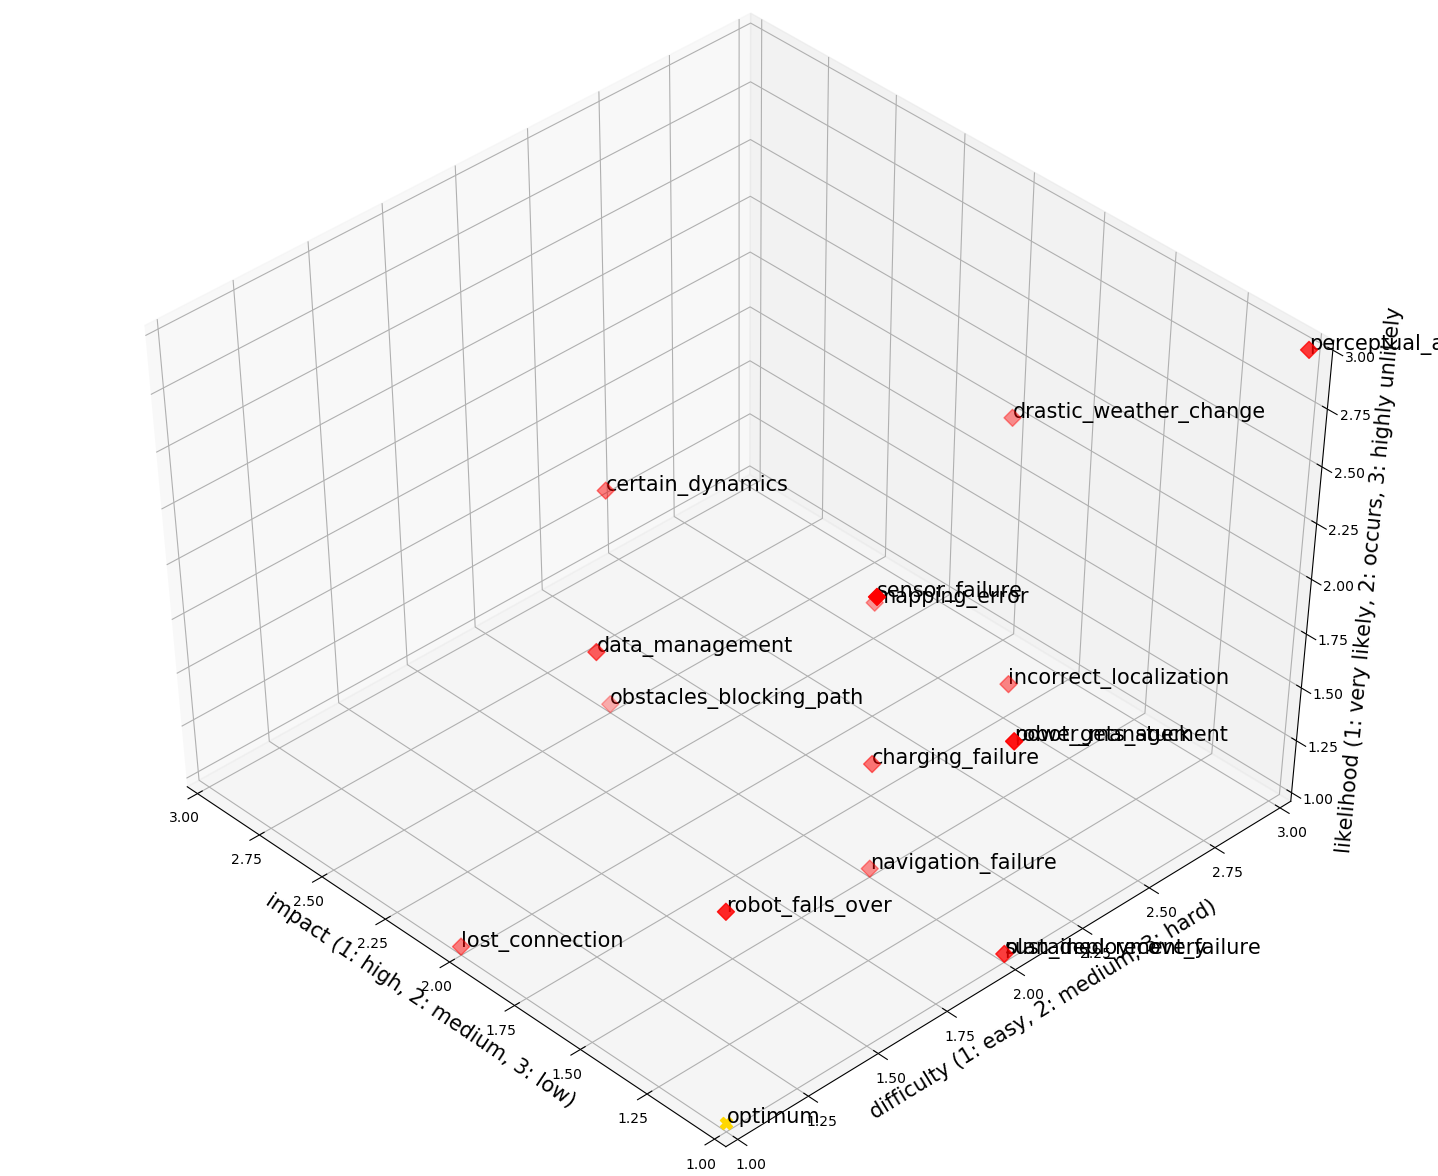
\includegraphics[width=0.95\textwidth]{pics/questionnaire.png}
    \caption{\textsc{Accumulated Results of Questionnaire}}
    \label{fig:questionnaire_results}
\end{figure}
\begin{figure}[H]
    \centering
    \resizebox{0.75\textwidth}{!}{
    \begin{tabular}{| c | c | c | c | c |}
        \hline
        \textbf{problem} & \textbf{\o \thinspace impact} & \textbf{\o \thinspace difficulty} & \textbf{\o \thinspace likelihood} & \textbf{dist. to optimum} \\ \hline
        charging\_failure & $1.29$ & $1.29$ & $1.71$ & $0.82$ \\ \hline
        power\_management & $1.0$ & $1.43$ & $2.0$ & $1.09$ \\ \hline
        data\_management & $1.57$ & $2.0$ & $1.86$ & $1.44$ \\ \hline
        sensor\_failure & $1.57$ & $1.71$ & $2.14$ & $1.46$ \\ \hline
        incorrect\_localization & $1.57$ & $2.29$ & $1.57$ & $1.52$ \\ \hline
        lost\_connection & $2.14$ & $1.86$ & $1.57$ & $1.54$ \\ \hline
        navigation\_failure & $1.86$ & $2.0$ & $1.83$ & $1.56$ \\ \hline
        plan\_deployment\_failure & $1.67$ & $1.83$ & $2.17$ & $1.58$ \\ \hline
        mapping\_error & $1.86$ & $2.14$ & $1.71$ & $1.6$ \\ \hline
        certain\_dynamics & $2.43$ & $1.43$ & $1.71$ & $1.65$ \\ \hline
        obstacles\_blocking\_path & $2.29$ & $2.14$ & $1.43$ & $1.77$ \\ \hline
        robot\_gets\_stuck & $1.43$ & $2.29$ & $2.14$ & $1.77$ \\ \hline
        sustained\_recovery & $1.33$ & $2.5$ & $2.0$ & $1.83$ \\ \hline
        drastic\_weather\_change & $1.86$ & $2.43$ & $2.29$ & $2.11$ \\ \hline
        robot\_falls\_over & $1.0$ & $2.33$ & $2.67$ & $2.13$ \\ \hline
        perceptual\_aliasing\_issue & $2.0$ & $2.5$ & $2.33$ & $2.24$ \\ \hline
    \end{tabular}}
\caption{\textsc{Results of the Evaluation - Problems Ordered by Relevance}}
\label{fig:average_results}
\end{figure}
\noindent
The results shown in the table in fig. \ref{fig:average_results} are ordered by their relevance according to the questionnaire results, i.e.
by their distance from the optimal combination of impact, difficulty, and likelihood. It is worth mentioning, however, that the resulting order is based on the assumption
that the three criteria of impact, difficulty, and likelihood are equally important in the consideration. One could argue that the difficulty criterion was introduced 
primarily because of the tight time frame of this work and may be less important when it comes to the question of which problem is really crucial to solve in practice.
Thus, it is worth considering the two-dimensional results only in terms of the expected impact and likelihood of each problem displayed in fig. \ref{fig:questionnaire_results_2d}.
\begin{figure}[H]
    \centering
    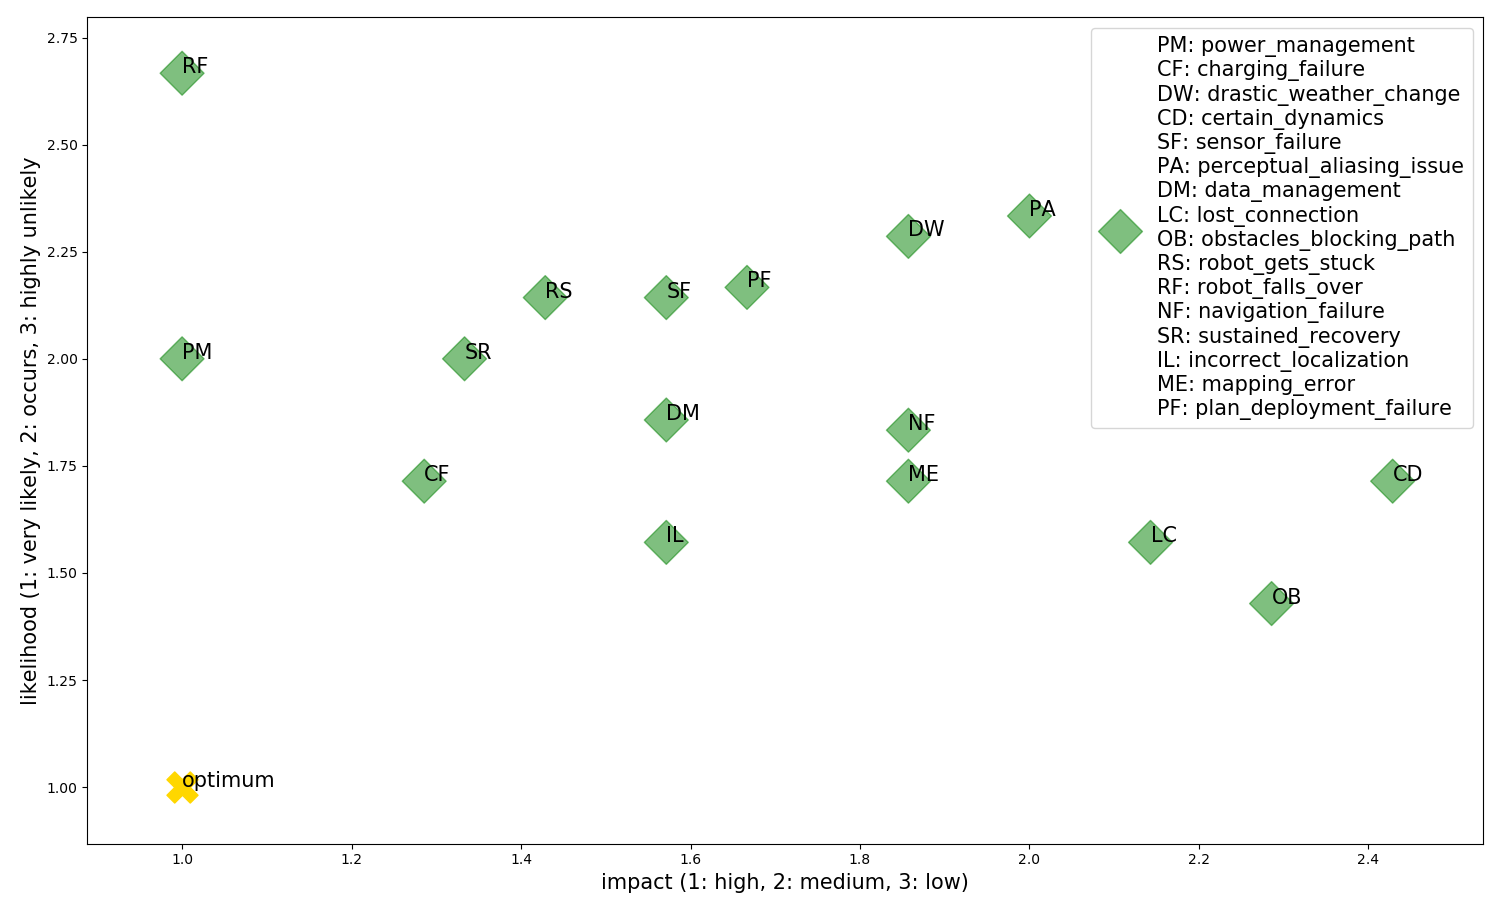
\includegraphics[width=0.7\textwidth]{pics/questionnaire_2d.png}
    \caption{\textsc{2D Results of Questionnaire}}
    \label{fig:questionnaire_results_2d}
\end{figure}
\noindent
Another interesting aspect to analyze is the range in given answers in the questionnaire, i.e. the agreement among the participants. Most of the judgments roughly coincide with
only few outliers. However, there are some controversial cases that are worth mentioning. First, the \textit{impact} category seems to be the easiest to assess, as it is the only
one where all participants agreed on two problem types (power management, robot falls over). In addition, the other problem types in the \textit{impact} category are rated fairly
consistently, most of them have only one outlier vote, and it is very rare that the votes are completely mixed. The most contested problem types in this category are perceptual
aliasing, connection losses, situations where the robot gets stuck, and navigation failures. It is also interesting to examine the reason for the mixed results. This could be
because most participants rated the problem as average on the scale, but it could also arise from extreme answers canceling each other out. There's a big difference - one means
participants agree, the other means they do not. For the \textit{impact} category, participants seem to agree overall, with only a few outliers and even some cases of perfect
agreement with unanimous votes. The next category, \textit{difficulty}, is already not so clear-cut, which may be explained by the fact that participants could imagine different
depths of problem-solving based on their particular experience, while \textit{impact} is quite easy to think about. There is no unanimous vote, and there are even some cases where
the answers are very mixed, such as in the case of lost connections, where the answers are almost evenly distributed among the possible options. However, this is still rare, in most
cases the overall trend is clear. Finally, the voting in the third category \textit{likelihood} is similar to the \textit{difficulty} votes. There is no unanimous vote, but there
are cases where participants are pretty much in agreement, such as in data management failures, where all but one voted for $2$ (\textit{occurs}). There is no extreme example of
evenly distributed responses, most have some tendency and a few outliers. In summary, an average score almost never results from an even distribution of responses across the options,
but almost always results from the actual rating of the problem as average based on the criteria. The exact results can be taken from the appendix 
(cf. \ref{sec:detailed_questionnaire_results}).\newline
As shown in fig. \ref{fig:average_results_2d}, the $2D$ evaluation purely based on impact and likelihood results in a different ordering based on their distances 
to the $2D$ optimum $(1, 1)$.
\begin{figure}[H]
    \centering
    \resizebox{0.65\textwidth}{!}{
    \begin{tabular}{| c | c | c | c | c |}
        \hline
        \textbf{problem} & \textbf{\o \thinspace impact} & \textbf{\o \thinspace likelihood} & \textbf{dist. to optimum} \\ \hline
        charging\_failure & $1.29$ & $1.71$ & $0.77$ \\ \hline
        incorrect\_localization & $1.57$ & $1.57$ & $0.81$ \\ \hline
        power\_management & $1.0$ & $2.0$ & $1.0$ \\ \hline
        data\_management & $1.57$ & $1.86$ & $1.03$ \\ \hline
        sustained\_recovery & $1.33$ & $2.0$ & $1.05$ \\ \hline
        mapping\_error & $1.86$ & $1.71$ & $1.12$ \\ \hline
        navigation\_failure & $1.86$ & $1.83$ & $1.2$ \\ \hline
        robot\_gets\_stuck & $1.43$ & $2.14$ & $1.22$ \\ \hline
        sensor\_failure & $1.57$ & $2.14$ & $1.28$ \\ \hline
        lost\_connection & $2.14$ & $1.57$ & $1.28$ \\ \hline
        plan\_deployment\_failure & $1.67$ & $2.17$ & $1.34$ \\ \hline
        obstacles\_blocking\_path & $2.29$ & $1.43$ & $1.36$ \\ \hline
        drastic\_weather\_change & $1.86$ & $2.29$ & $1.55$ \\ \hline
        certain\_dynamics & $2.43$ & $1.71$ & $1.6$ \\ \hline        
        robot\_falls\_over & $1.0$ & $2.67$ & $1.67$ \\ \hline
        perceptual\_aliasing\_issue & $2.0$ & $2.33$ & $1.67$ \\ \hline
    \end{tabular}}
\caption{\textsc{Results of the $2D$ Evaluation - Problems Ordered by Relevance}}
\label{fig:average_results_2d}
\end{figure}
\noindent
First, it is interesting to note that the charging failure is undisputedly in first place in both the two-dimensional and three-dimensional evaluations.
The problem of incorrect localization climbs to second place if the difficulty criterion is disregarded. This is followed, as before, by power and data management.
Subsequently, sustained recovery makes a huge jump of eight places when leaving aside its assumed difficulty to detect and solve.
Mapping errors are also on the rise, overtaking sensor failures, lost connections, navigation failures, and plan deployment errors.
Another interesting aspect is that sensor failures are far less relevant when disregarding their surprisingly low rated difficulty.
The remaining problems remain broadly similar in their assessment, with some changing places in the middle of the list, but this is not so relevant.
The problems rated as least relevant in the questionnaire remain the same as in the 3D case, mainly because they are considered relatively unlikely.
In conclusion, both lists are used to prioritize the problems to be studied in this work, as it is of course useful to also consider the difficulty of 
solving these problems, but the $2D$ view can be helpful in case of doubt.

\pagebreak

\noindent
\textbf{Systematization of LTA-Challenges}\newline

\noindent
It would be beyond the scope of this work to tackle every identified potential challenge for a mobile robot's long-term autonomy. Therefore, it is necessary to select a subset of the
problems to be considered based on the results of the questionnaire. For this subset, monitoring methods are presented that do not necessarily solve $100\%$ of the possible cases,
but a certain fraction, at least to a first approximation. In addition, more fundamental problems are emphasized that cannot be addressed in general within the scope of this work;
special cases may be. 
First, it is obvious that charging failures should be addressed in this work, since they are undisputedly in the first place in both the two-dimensional and three-dimensional
evaluations of the questionnaire (cf. \ref{sec:sim_charging_failures}, \ref{sec:mon_charging_failures}). Thematically closely related and also very relevant based on the survey:
power management problems (cf. \ref{sec:sim_power_management}, \ref{sec:mon_power_management}). Another aspect high on the list to be considered in this work is data management
issues (cf. \ref{sec:sim_data_management}, \ref{sec:mon_data_management}). Furthermore, sensor (perception) failures are a class of problems that should not be ignored in this work
(cf. \ref{sec:sim_sensor_failures}, \ref{sec:mon_sensor_failures}). Although in principle a very intricate and general class of problems, localization issues, i.e. incorrect
localization (cf. \ref{sec:sim_incorrect_localization}, \ref{sec:mon_incorrect_localization}), has to be considered in this work, especially due to its high impact and likelihood
that can be seen in fig. \ref{fig:average_results_2d}. Additionally, connection problems are treated (cf. \ref{sec:sim_lost_connections}, \ref{sec:mon_lost_connections}). Also quite
general, but pretty high on the list are navigation errors, which are taken into account at least to some degree (cf. \ref{sec:sim_navigation_failures}, 
\ref{sec:mon_navigation_failures}). Being relatively easy to detect, plan deployment failures will be tackled as well (cf. \ref{sec:sim_plan_deployment_failures},
\ref{sec:mon_plan_deployment_failures}). Although the problem of obstacles blocking the robot's path is ranked quite low in the lists in figs. \ref{fig:average_results} and
\ref{fig:average_results_2d}, it is considered to some extent because the reason for its low ranking is mainly its relatively small impact. However, it is rated as very likely,
and it would be good if such situations could be dealt with effectively (cf. \ref{sec:sim_obstacles}, \ref{sec:mon_obstacles}). The problem of sustained recovery is fairly low on
the list in the $3D$ assessment, but very high in the $2D$ case, mainly because of its relatively large impact. Thus, it will be studied (cf. \ref{sec:sim_sustained_recovery},
\ref{sec:mon_sustained_recovery}). The issue of drastic weather changes is rated as rather irrelevant in the overall result of the questionnaire. However, this is mainly due to
its high rated difficulty and the relatively low likelihood. Although it may be difficult to solve in general, it will be dealt with in first approximation due to its quite high
impact (cf. \ref{sec:sim_drastic_weather}, \ref{sec:mon_drastic_weather}).\newline
A not so high-rated and also very general problem class that is not considered in detail in this work: Mapping errors. The problem class ``certain dynamics'' is of course formulated
quite generally in the questionnaire, which could be one of the reasons for the low impact rating, but for this work dynamics like sunset are not further investigated as they are
quite predictable. In addition, situations in which the robot gets stuck are not taken into account because they are regarded relatively irrelevant due to their low probability.
Of course, it is a severe problem when it happens, but the robot actually getting completely stuck is relatively rare, and due to the many possible reasons for getting stuck, 
a very general problem class. All participants agree that the scenario where the robot topples over has a very large impact, but it is also quite difficult to detect and quite
unlikely. It is not studied in detail itself, but might be detected as part of the sensor failure detection, e.g. if the sensor subsequently points to the sky (cf.
\ref{sec:mon_sensor_failures}). Finally, ranked as least relevant in both evaluations, perceptual aliasing issues will be disregarded in this work. The problems not examined in
detail in this thesis are nevertheless potentially relevant problems for the long-term autonomy of a mobile outdoor robot and are thus briefly discussed in section 
\ref{sec:lta_problems_not_considered}.

\subsection{LTA Problems Not Considered in this Work}
\label{sec:lta_problems_not_considered}

\noindent
\textbf{Certain Dynamics}\newline

\noindent
There should be a monitoring solution that is able to detect twilight, stop the plan execution and postpone it to the next day.\newline
It should be possible to simulate twilight in the Gazebo simulation, e.g. by simply dimming the light source.

\noindent
\textbf{Perceptual Aliasing Issue}\newline

There could be a need for monitoring methods that are capable of recognizing such situations and providing some strategies to resolve the 
perceptual aliasing issue., e.g. by changing the position or the viewpoint in order to discriminate the objects.\newline
The occurrence of a perceptual aliasing issue can be simulated, for example, by placing an object similar to the container in the simulation.

\noindent
\textbf{Robot Gets Stuck}\newline

\noindent
Detection should be based on \code{move\_base\_flex} recovery behaviors, as in the case of obstacles, but again there should be a manual implementation 
specifically for these cases where, for example, the robot tries to rotate and reduce speed to leave the place where it got stuck.\newline
In simulation, such a situation could be established by providing the necessary physical conditions leading to such a problem.\newline

\noindent
\textbf{Robot Falls Over}\newline

\noindent
It could be tested in simulation by applying a force to the robot that causes it to fall over.\newline
It should be possible to detect the problem based on a combination of sensor information, and the robot should notify the human operator.

\noindent
\textbf{Mapping Issues}\newline

\noindent
It is demanded to either pay close attention to obstacle detection when moving on uneven terrain or to clear the \textit{costmap} from time to time
to eliminate such erroneous entries. This is especially true for recovery behaviors,  where such ``virtual'' objects can block a path that the robot must traverse.\newline
The problems described can be evaluated in simulation by having the robot travel over rough terrain or by artificially creating paths with steep inclines.

\chapter{Plan Execution and Monitoring}

A key aspect of handling some of the potential issues introduced in section \ref{sec:challenges_for_lta} is going to be that the robot will not be able to
complete its missions without preempting the plan execution from time to time. Either due to insufficient battery capacity or other unmanageable conditions such as 
drastic weather changes that force the robot to interrupt its task. Although the overall route may always be the same for the same field, there are certain stopping
conditions that cause the robot to interrupt its active scanning tour and possibly drive back to its base, i.e. the mobile container.
There are generally two relevant perspectives. First, such stops have to be considered at planning time by acknowledging charge stops as crucial part of the plan.
Of course, this is only covering plannable stops such as expected battery consumption and is not able to deal with unplanned situations.
Therefore, a second perspective comes into play, that will be particularly relevant in this work - the execution time.
Just as important as the planning itself is the execution of the generated plan as well as monitoring the execution.
The idea is that the robot executes a given plan and is somehow capable of realizing that it has to interrupt the execution due to some unexpected condition.
In such a case, the robot needs to be able to save the current state of the plan execution and continue precisely with this state after the reason 
for the interruption has been resolved. Consequently, the robot has to be prepared to pause and resume the execution of a given plan, which is far from 
trivial, since the original plan may no longer be applicable for various reasons.

\section{Execution Monitoring State Machine Architecture}
\label{sec:execution_monitoring_smach_architecture}

Plan execution as well as robot operation monitoring are modeled as a high-level hierarchically structured state machine, whose architecture is shown
in figure \ref{fig:high_level_smach}. The architecture is implemented using the SMACH\footnote{ROS-independent Python library to build hierarchical state machines \cite{smach}} 
library.
\begin{figure}[H]
    \centering
    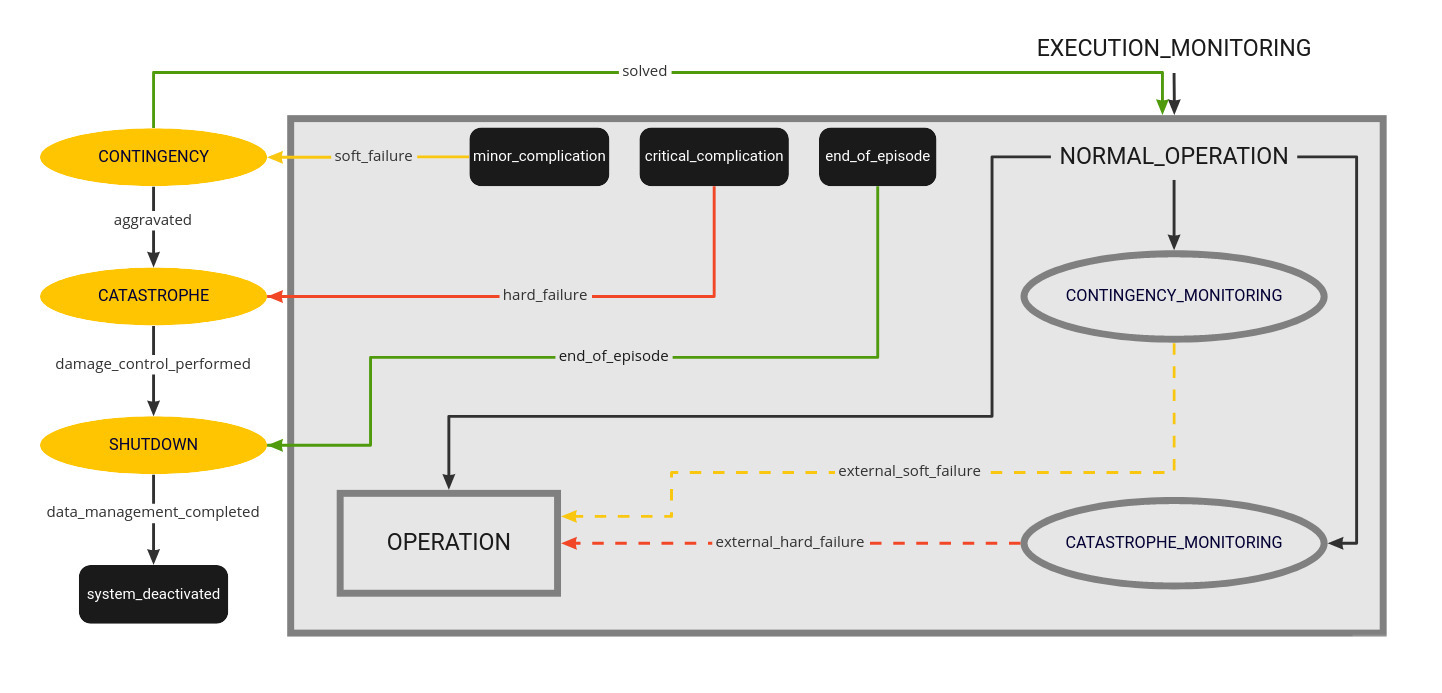
\includegraphics[width=\textwidth]{pics/SMACH_high_level.jpg}
    \caption{\textsc{Architecture of the Hierarchical State Machine (High-Level)}}
    \label{fig:high_level_smach}
\end{figure}
\noindent
As depicted in figure \ref{fig:high_level_smach}, the robot starts in the state \code{NORMAL\_OPERATION} in the high-level hierarchical state machine \code{EXECUTION\_MONITORING}.
\code{NORMAL\_OPERATION} is represented by an embedded state machine named \code{OPERATION}, visualized in figure \ref{fig:low_level_smach}, as well as the two
parallel running execution monitoring states (cf. ROS \code{MonitorState} \cite{monitor_state}) \code{CONTINGENCY\_MONITORING} and \code{CATASTROPHE\_MONITORING}, 
implemented as a concurrence container (cf. SMACH \code{Concurrence} \cite{concurrence_container}).
These parallel running states are used to monitor the robot's operation and to interrupt it when a problematic situation requiring special treatment is detected
(see the dashed arrows in figure \ref{fig:high_level_smach}).
Although a monitoring solution could in principle also be implemented sequentially, it seems more natural to choose a parallel approach, since a sequential option
would have the disadvantage that no monitoring takes place while a task / algorithm is being executed, but only afterwards.
It is desirable to be able to intervene at any time during the execution of a task when a monitoring procedure running in parallel is triggered and causes a change of state.
During the state \code{OPERATION}, i.e. in the nested state machine visualized in figure \ref{fig:low_level_smach}, the robot can be either in the state \code{IDLE}, 
in which it is waiting for a plan, or in \code{EXECUTE\_PLAN}, in which it is executing a given plan. The embedded state machine \code{OPERATION} has 
four possible outcomes - \code{end\_of\_episode}, \code{minor\_complication}, \code{critical\_complication}, and \code{preempted}. 
It starts in the \code{IDLE} state and remains there as long as no plan is provided via a ROS service.
There are two common options for the robot to leave the state. The first is via a message on a ROS topic indicating that the end of the current long-term episode
has been reached, resulting in an overall outcome of \code{end\_of\_episode} for \code{NORMAL\_OPERATION}. The second is to receive a plan that results in a state
transition to \code{EXECUTE\_PLAN}. Additionally, the external parallel running monitoring states \code{CONTINGENCY\_MONITORING} and \code{CATASTROPHE\_MONITORING}
are capable of interrupting the \code{IDLE} state at any time (cf. state preemption \cite{state_preemption}) due to external problems leading to the outcome \code{preempted}.
In \code{EXECUTE\_PLAN}, there are five possible outcomes, two of which result in state transitions and three of which cause \code{OPERATION} 
to return to the parent state machine. The first possible outcome is \code{action\_completed}, which indicates that an action of the currently processed plan was 
completed successfully and causes the same state (\code{EXECUTE\_PLAN}) to be executed again with the reduced plan, i.e. the rest of the plan is executed.
The next possible outcome is \code{plan\_completed}, which means that the entire plan has been successfully processed and causes a transition back to the \code{IDLE} state.
These were the possible outcomes that cause a transition to another state. Now there are the three remaining outcomes that cause a return to the parent state machine. 
First, \code{soft\_failure}, which means that something went wrong, e.g. an action was not performed successfully, but the robot should be able to handle the problem. 
Second, there is the potential outcome \code{hard\_failure}, which represents situations where the robot is unable to solve the problem itself.
Finally, the last potential outcome is again \code{preempted} based on some external issue detected by \code{CONTINGENCY\_MONITORING} or \code{CATASTROPHE\_MONITORING}.
\begin{figure}[H]
    \centering
    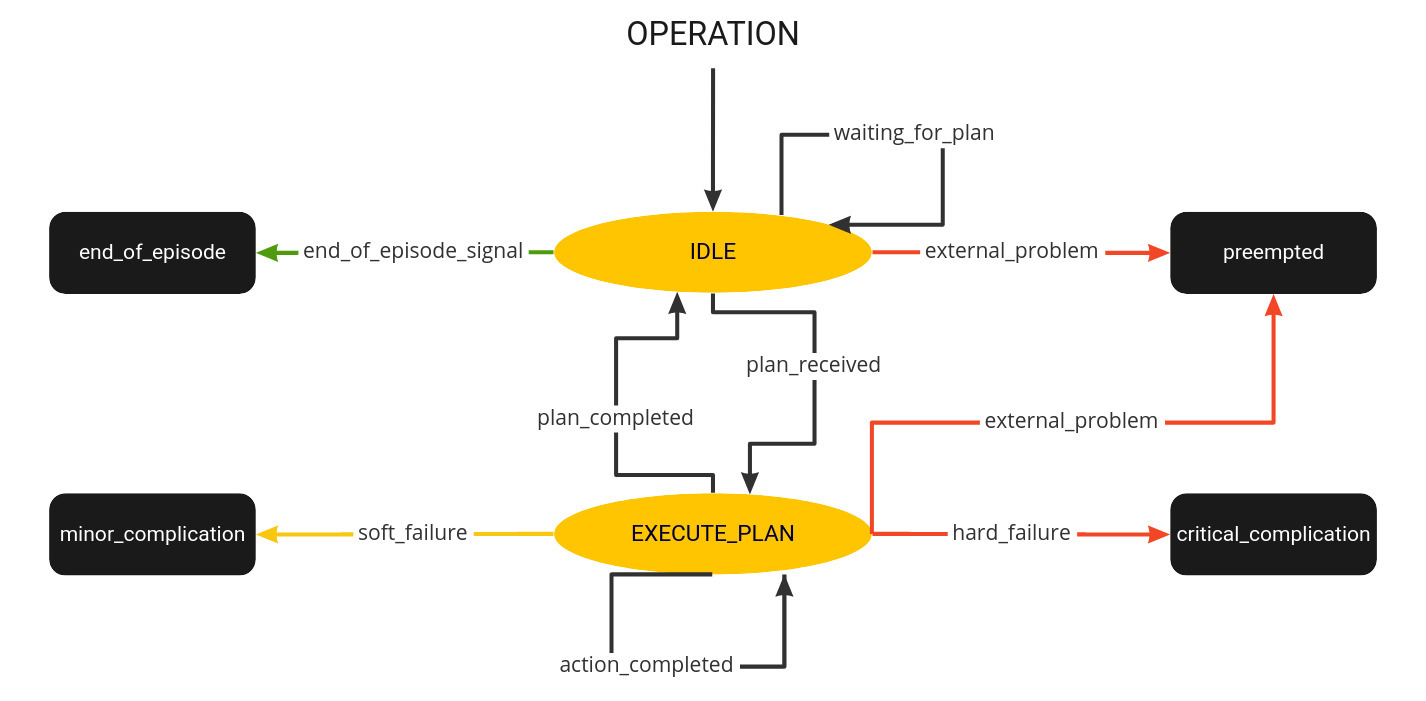
\includegraphics[width=\textwidth]{pics/SMACH_low_level.jpg}
    \caption{\textsc{Architecture of the Embedded State Machine (Low-Level)}}
    \label{fig:low_level_smach}
\end{figure}
\noindent
Now that the control flow of \code{NORMAL\_OPERATION} and, in particular, \code{OPERATION} has been clarified, we return to the parent state machine shown 
in figure \ref{fig:high_level_smach}.
As mentioned, when \code{NORMAL\_OPERATION} returns \code{end\_of\_episode}, the parent state machine transitions to the \code{SHUTDOWN} state and the 
robot's work for that long-term episode is complete, which means that the robot performs data management and then the system is deactivated.
Essentially, in a long-term episode in the considered scenario, the robot should stay in \code{NORMAL\_OPERATION} as 
long as the episode is running or an error / problem has occurred, either an error that it is able to deal with itself or even a more severe problem that requires the 
intervention of a human operator. Accordingly, if \code{NORMAL\_OPERATION}, i.e. the embedded state machine together with the parallel running monitoring states has the outcome 
\code{minor\_complication}, the robot enters the state \code{CONTINGENCY}, which means that it has detected a soft failure, e.g. a sensor failure, but its ability to act
is preserved, it is for example able to drive back to the base in safety mode. However, if \code{NORMAL\_OPERATION} returns \code{critical\_complication}, there is a hard 
failure that is unsolvable for the robot, perhaps even for the operator, and the robot transitions to \code{CATASTROPHE}. If it is still possible, the robot saves the current 
state of the plan execution, sends an emergency signal, e.g. communicates the problem to the operator, and shuts down, i.e. transitions to \code{SHUTDOWN}.
There are, of course, situations in which the robot can no longer do anything, such as when the battery is completely discharged.
In principle, such cases also fall under the category of catastrophe, but since monitoring then no longer works, there is nothing left to do there.
Besides, there are two more transitions depicted in figure \ref{fig:high_level_smach}: From \code{CONTINGENCY} back to \code{NORMAL\_OPERATION}, after a minor problem is resolved by the robot, it can continue
its normal operation. Additionally, it is possible that something goes wrong during \code{CONTINGENCY} or that the problem actually cannot be solved by the robot,
such that it transitions to \code{CATASTROPHE}.\newline
To be clear, \code{NORMAL\_OPERATION} can manage problems in two ways.
First, a problem may occur during plan execution in the child state machine, in such a case \code{OPERATION} returns \code{critical\_complication} or 
\code{minor\_complication} to the parent state machine based on the problem severity and a corresponding state transition takes place.
In addition, there are the described parallel monitoring states, which are responsible for problems that are not directly related to plan execution, but are of a more general nature.
If these detect a problem, they are able to interrupt \code{OPERATION} and also return \code{critical\_complication} or \code{minor\_complication} to the parent state machine
\code{EXECUTION\_MONITORING}. It is trivial to interrupt \code{OPERATION} when no task is currently being executed, i.e. no scan is being recorded and no navigation target 
is being approached. However, it is obvious that potential problems do not wait for the completion of such tasks, but can also occur during the execution of an action.
Therefore, the \code{drive\_to$(lat, lng, \theta)$} and \code{scan} actions are implemented as ROS \code{SimpleActionClient}s that can be interrupted at any time
by calling the \code{cancel\_all\_goals()} method, which immediately interrupts all running goals. It is quite important that the robot is able to preempt the plan 
execution at all times, e.g. does not continue to drive to its goal, but should instantly stop the \code{move\_base\_flex} goal execution and start following the
recovery instructions.\newline
The general difference between the \code{CONTINGENCY} and \code{CATASTROPHE} states is the robot's ability to act. 
In a catastrophe case, it is no longer really capable of acting in the sense of driving back to its base, managing the problem itself, etc. 
An example for a catastrophic case would be that the robot falls over. It is then unable to recover, but it is of course still able to communicate the problem
and save the state, in full possession of its ``mental'' powers, so to speak. Whereas a lightning strike, as an extreme example, could cause the robot to have a 
complete breakdown and nothing to work at all. The boundaries there are not quite sharp, there are many edge cases.
The following somewhat more mundane example, considering the robot's battery, will illustrate the concepts.
In \code{NORMAL\_OPERATION}, the battery discharges according to the plan. There may be some fluctuations due to temperature, for example, but it works roughly as expected.
It would transition to the state \code{CONTINGENCY} when it detects that the battery is already too low to complete the plan, but it is still able to recover,
i.e. drive back to its base, recharge, and continue the plan execution. However, it would proceed to \code{CATASTROPHE} if it detects that the battery is so low
that it can already tell that it is not possible to reach the base and recharge. It is then still able to communicate the problem and save the state, but it is not able
to recover. The extreme case, where nothing can be done, would be that the battery suddenly just breaks.

\pagebreak

\section{Plan Generation and Format}
\label{sec:plan_generation}

Long-term autonomous robot operation commonly includes following some sort of plan. However, since the actual planning is not part of this work, it is assumed that
plans are provided and usable, e.g. handcrafted by a human operator or generated by a planner from the literature.
For the purpose of parsing such plans and making them retrievable via a service call, a ROS node was developed.
In order for the node to parse the plans, they must be formulated in the following CSV format.
There are four available actions - \code{drive\_to$(lat, lng, \theta)$}, \code{return\_to\_base}, \code{charge}, and \code{scan}.
Each line in the CSV file represents one action of the plan. The actions \code{return\_to\_base}, \code{charge} and \code{scan} have no parameters,
but \code{drive\_to$(lat, lng, \theta)$} needs the additional arguments latitude, longitude, and orientation of the target pose.
An example for a simple plan is shown in figure \ref{fig:plan_example}. 
When the robot executes this plan, it drives to the four specified locations in sequence and records scans.
Afterwards, it returns to the base and recharges its battery.
\begin{figure}[H]
    \centering
    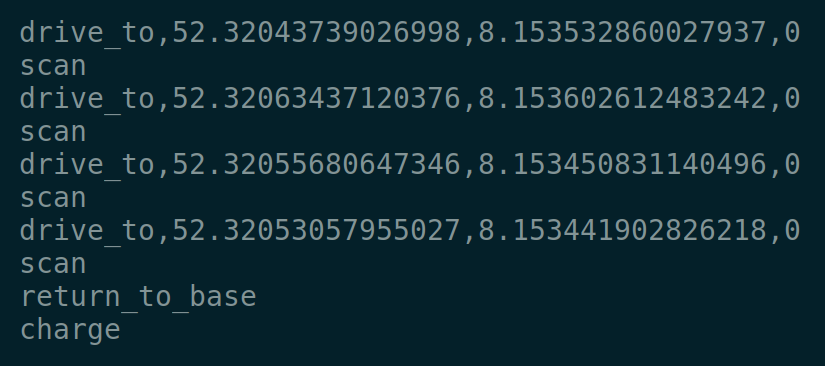
\includegraphics[width=0.5\textwidth]{pics/plan_example.png}
    \caption{\textsc{Sample Plan}}
    \label{fig:plan_example}
\end{figure}
\noindent

\section{Interrupt and Resume Normal Operation}

In order to handle unexpected problematic situations, the robot must be able to stop and resume its normal operation in general
and plan execution in particular, i.e. to save the current state of the plan execution and resume exactly that state after the reason
for the interruption has been resolved. The idea is that whenever the monitoring procedures \code{CONTINGENCY\_MONITORING} and \code{CATASTROPHE\_MONITORING} 
introduced in section \ref{sec:execution_monitoring_smach_architecture}, or the plan execution itself, detect a problem, they should trigger such an interruption.
As seen in the last section, there are two states in \code{OPERATION} that the robot can be in during a long-term episode without any problems
- \code{IDLE} or \code{EXECUTE\_PLAN}. In the \code{IDLE} state, where it waits for the plan generator described in section \ref{sec:plan_generation} to provide a plan,
it is straightforward, the normal operation is interrupted, the high-level state machine transitions to \code{CONTINGENCY} or \code{CATASTROPHE} depending
on the severity of the problem, and then, i.e. when the minor problem is resolved, it transitions back to \code{IDLE} or, in the case of \code{CATASTROPHE},
it shuts down. The more interesting case, of course, is such an interruption of normal operation when the robot is in the low-level state \code{EXECUTE\_PLAN}.
During the \code{EXECUTE\_PLAN} state, the currently executed plan is always stored in the \code{userdata} field of the state.
SMACH states always provide so-called \code{userdata} fields, which are essentially the input and output data of a SMACH state.
Initially, when \code{IDLE} receives a plan from the plan generator, it passes it as \code{userdata} to the \code{EXECUTE\_PLAN} state.
Then, whenever \code{EXECUTE\_PLAN} successfully completes an action of the plan, the reduced plan is passed to the next iteration of the same state.
Therefore, based on this architecture, the current state of the plan execution is always stored in the \code{userdata} of the SMACH. To comply with this fact, a certain situation
must be handled. If a plan execution is interrupted during the execution of an action, this action is already removed from the \code{userdata}, and since the execution of this
action must be repeated when the normal operation resumes, the action that was executed during the error must be reattached to the \code{userdata} before transitioning
to \code{CONTINGENCY} or \code{CATASTROPHE}.
Of course, when the robot transitions back to \code{NORMAL\_OPERATION} after solving a contingency, it starts again in \code{IDLE}, which is why \code{IDLE}
always looks for existing unfinished plans in the \code{userdata} first. If there is one, it does not prompt the plan generator for a new plan, but continues the previously
preempted plan. The catastrophe case works analogously to the \code{IDLE} state.

\section{Simulation of LTA Challenges}
\label{sec:simulation_of_lta_challenges}

In the following, potential ways of simulating each issue in order to evaluate it are discussed.

\subsection{Power Management}
\label{sec:sim_power_management}

Power management problems can be simulated quite easily based on a controllable battery consumption model that can be manipulated at will.

\subsection{Charging Failure}
\label{sec:sim_charging_failures}

A failed charging process is again quite easy to simulate based on a controllable battery consumption model such as the one explained in the previous paragraph.

\subsection{Drastic Weather Change}
\label{sec:sim_drastic_weather}

Although such weather conditions are difficult to simulate realistically, it might be worthwhile to implement at least a subset of them in the Gazebo
simulation to get an idea of how to detect them. But even if that is not realistically feasible within the scope of the work, there would be a second
option, in which the robot does not detect extreme weather conditions itself through its sensors, but simply relies on external local weather information.

\subsection{Sensor (Perception) Failure}
\label{sec:sim_sensor_failures}

The evaluation of a total sensor failure is straightforward, as it can be easily simulated by interrupting the publication of laser scans in the dummy scanning node
described in section \ref{sec:dummy_scanning_node}. The second identified type of sensor failure, i.e. an empty list of range values, is again rather trivial to simulate
by clearing the list of range values before republishing a scan in the dummy scanning node. Scans consisting mainly of impermissible range values can be realized by 
simply manipulating the range values of a scan so that they do not satisfy the maximum and minimum range of the sensor before republishing, i.e. \code{inf}.
Finally, to simulate repeated scans, the dummy scanning node always stores the previous scan and can replace the current scan with the previous one on command.
Accordingly, the simulation of each different sensor fault case is implemented as part of the dummy scanning node introduced in section \ref{sec:dummy_scanning_node},
and can be enabled / disabled via the following ROS topics:
\begin{itemize}
    \item \textbf{total sensor failure} \textrightarrow \code{/toggle\_simulated\_total\_sensor\_failure}
    \item \textbf{empty list of range values} \textrightarrow \code{/toggle\_simulated\_empty\_ranges}
    \item \textbf{predominantly impermissible values} \textrightarrow \code{/toggle\_simulated\_impermissible\_ranges}
    \item \textbf{repeated scan} \textrightarrow \code{/toggle\_simulated\_scan\_repetition}
\end{itemize}

\subsection{Data Management}
\label{sec:sim_data_management}

It is not a big challenge to simulate the occurrence of the data management problems presented in section \ref{sec:challenges_for_lta}. To simulate a ``full disk''-failure,
i.e. a full memory of the drive on which the scans are to be logged, one could simply prepare a full USB flash drive and configure the path to be monitored accordingly,
e.g. mount flash drive to \code{/mnt/usb} and set \code{MONITOR\_DRIVE = /mnt/usb}. The second and more scenario-specific type of error is the scan logging error, which
can be simulated by simply not writing the scan to the file system in the dummy scanning node introduced in section \ref{sec:dummy_scanning_node}. Simulation of this type
of error can be enabled / disabled via the ROS topic \code{/toggle\_simulated\_scan\_logging\_failure}.

\subsection{Lost Connection}
\label{sec:sim_lost_connections}

\subsubsection{WiFi Connection Failures}
\label{sec:sim_wifi_connection_problems}

The simulation of WiFi connection failures is realized by the operating-system-specific implementation of a WiFi monitoring node described in section
\ref{sec:monitoring_for_lta_challenges}. The idea is to simply publish problematic values for each of the considered attributes of the WiFi connection,
i.e. link quality, signal level and bit rate. The simplest case of a complete disconnection is simulated by setting all three values to $0$.
Since the question of which values are considered problematic depends heavily on the environment and application scenario, these values are configurable by the user.
By default, a poor link is simulated by publishing a corresponding value of $2\%$, meaning that the measure of how good the link is described in section
\ref{sec:challenges_for_lta} estimates the quality with only two percent of the optimum. The second attribute, the received signal strength indication (RSSI),
ranges from $-30$ dBm to $-100$ dBm, depending on various aspects, such as distance. \cite{Heurtefeux:2012} The upper bound of $-30$ dBm is the optimal value, which
is almost impossible to achieve in practice, and $-100$ dBm basically means no signal at all. One could roughly classify it as follows: Anything between the optimal
$-30$ dBm and $-67$ dBm can be considered very good in practice, below an RSSI of $-80$ dBm it starts to become critical, and around $-90$ dBm it becomes practically 
unusable. \cite{metageek} Thus, a signal level failure is simulated by publishing an RSSI value of $-90$ dBm. Finally, the default value for a simulated bit rate failure 
is $0.1$ Mb/s. The simulation of each different WiFi fault case can be enabled / disabled via the following ROS topics:
\begin{itemize}
    \item \textbf{poor link quality} \textrightarrow \code{/toggle\_simulated\_bad\_wifi\_link}
    \item \textbf{poor signal level} \textrightarrow \code{/toggle\_simulated\_bad\_wifi\_signal}
    \item \textbf{poor bit rate} \textrightarrow \code{/toggle\_simulated\_bad\_wifi\_bit\_rate}
    \item \textbf{disconnection} \textrightarrow \code{/toggle\_simulated\_wifi\_disconnect}
\end{itemize}

\subsection{Obstacles Blocking the Planned Path}
\label{sec:sim_obstacles}

The occurrence of static and dynamic obstacles can be implemented in the simulation by spawning mobile and immobile objects at randomized 
positions that could potentially block the robot's path.

\subsection{Navigation Failure}
\label{sec:sim_navigation_failures}

Problems of this type could be evaluated in simulation through specially constructed examples that are particularly difficult for the navigation algorithms to solve.

\subsection{Sustained Recovery}
\label{sec:sim_sustained_recovery}

Sustained recoveries can be evaluated in the simulation by inducing situations where recovery is not possible, such as when the path to the destination is
blocked and there is no other way.

\subsection{Incorrect or Inaccurate Localization}
\label{sec:sim_incorrect_localization}

An incorrect localization can be evaluated very well in the simulation by simply ``teleporting'' the robot to another position, i.e. provoking the
\textit{kidnapped robot problem}.

\subsection{Plan Deployment Failure}
\label{sec:sim_plan_deployment_failures}

The problem can be trivially simulated by simply not launching the plan generation service.

\section{Monitoring for LTA Challenges}
\label{sec:monitoring_for_lta_challenges}

Now that the overall architecture of the execution monitoring state machine has been described (cf. section \ref{sec:execution_monitoring_smach_architecture}), we can turn to the
actual monitoring methods for the potential hinderances for long-term autonomous systems introduced in section \ref{sec:challenges_for_lta}. The idea is to implement a specific
monitoring procedure for each of the presented LTA problems that runs in parallel to the high-level state machine. Whenever such a procedure is triggered, i.e. the specific issue
is recognized, the problem gets reported via the \code{MonitorState}s, causing a transition to \code{CONTINGENCY} or \code{CATASTROPHE} based on the severity of the problem.
Depending on the nature of the problem, the information about the required solution method is conveyed via the message published to the topic of the \code{MonitorState}.
Thus, the overall goal is to have a resolver node for each of the potential failures, which is executed in \code{CONTINGENCY} or \code{CATASTROPHE} depending on the
failure case at hand. The entire process is essentially the same for all potential LTA problems - fault simulation, monitoring, and subsequent remediation.
Initially, it will be demonstrated that in the prototypical scenario, the mission can no longer be completed successfully if these errors occur.
After launching the monitoring nodes, the problems should be detected and either resolved by the robot or reported to the operator so that the mission can continue.
The simulated failures are implemented in such a way that they can be triggered by publishing to a certain topic.

\subsection{Power Management}
\label{sec:mon_power_management}

A watchdog module that monitors the battery state and acts as a fail-safe, such as the one described in section \ref{sec:battery_monitoring}, could be 
integrated to address power management issues and improve the robot's survivability.

\subsection{Charging Failure}
\label{sec:mon_charging_failures}

Both cases should be detected by the robot so that an appropriate response can be initiated, e.g. notification of the human operator. The first case, i.e. a docking 
failure, could for example be detected based on \code{move\_base\_flex} navigation errors, the docking state simply does not complete successfully, which should trigger
a treatment procedure. A failed charging process can be detected based on a certain time in the state of charge without increasing the charge level of the battery.

\subsection{Drastic Weather Change}
\label{sec:mon_drastic_weather}

As described in the section on simulations, there are two ways to incorporate weather information, either by having the robot detect it with its own sensors or by 
utilizing external weather information. In any case, it would be good to identify extreme weather conditions that could affect the proper functioning of the system 
in order to react accordingly, i.e. return to the base station and seek shelter.

\subsection{Sensor (Perception) Failure}
\label{sec:mon_sensor_failures}

Executing a \code{scan} action not only launches the dummy scanning node introduced in section \ref{sec:dummy_scanning_node}, but also a monitoring procedure that
looks for potential problems with the laser scanner. The most obvious type of sensor failure is of course a total failure, i.e. no messages arrive on the corresponding ROS topic.
A fairly trivial approach to detecting total sensor failures is therefore to use \code{rospy.wait\_for\_message()} with the particular topic and set a time period
after which a missing scan is considered a total sensor failure. Of course, such a timeout is highly dependent on the respective application and also on the sensor 
configuration, since a higher angular resolution naturally requires a longer runtime, e.g. a longer runtime due to a higher resolution should not be falsely identified 
as sensor failure. In addition, there could be different modalities of recording with the sensor. The scan can be recorded continuously or published in parts.
Therefore, the time limit is configurable by the user. While trivial, such a monitoring is not yet available and is critical for reasonable long-term autonomy in the 
considered scenario described in section \ref{sec:prototype_scenario}. Nonetheless, more subtle errors should also be detected, beyond the outright absence of scans.
For this purpose, the incoming scans must be examined more closely and checked for plausibility. For example, if the list of range values is empty, it is as useless for
the mission as a scan that does not arrive at all. Hence, after the arrival of a new scan, the monitoring solution verifies that the list of range values is not empty.
Another interesting issue to detect is a list of range values that predominantly contains \code{inf} values, which, as mentioned in section
\ref{sec:simulation_of_lta_challenges}, could indicate that the sensor is pointing towards the sky, e.g. because the robot has fallen over,
or the sensor has slipped. Admittedly, it would be a bit too simplistic to consider only range lists entirely filled with \code{inf} values as problematic.
In many cases, depending on the field of view, the sensor can still receive reasonable values if it is oriented towards the sky, for example.
In the minimal simulation scenario with the AROX (see section \ref{sec:prototype_scenario}), the \textit{Velodyne} scanner still receives about $10$\% of 
reasonable-looking range values when the robot is tilted on its back and the sensor is pointing toward the sky, as shown in figure \ref{fig:tilted_AROX}.
As can be seen in figure \ref{fig:straight_line}, in such a case the sensor detects parts of the ground on both sides of the robot as well as parts of the 2.5D 
representation of a hedge in the background. Accordingly, it makes much more sense to let the user define a lower bound for reasonable-looking values (non-\code{inf}),
e.g. that depending on the scenario and sensor configuration at least $10$\% of the detected values must be non-\code{inf} for the scan to be considered feasible.
\begin{figure}[H]
    \centering
    \begin{subfigure}[b]{0.49\textwidth}
        \centering
        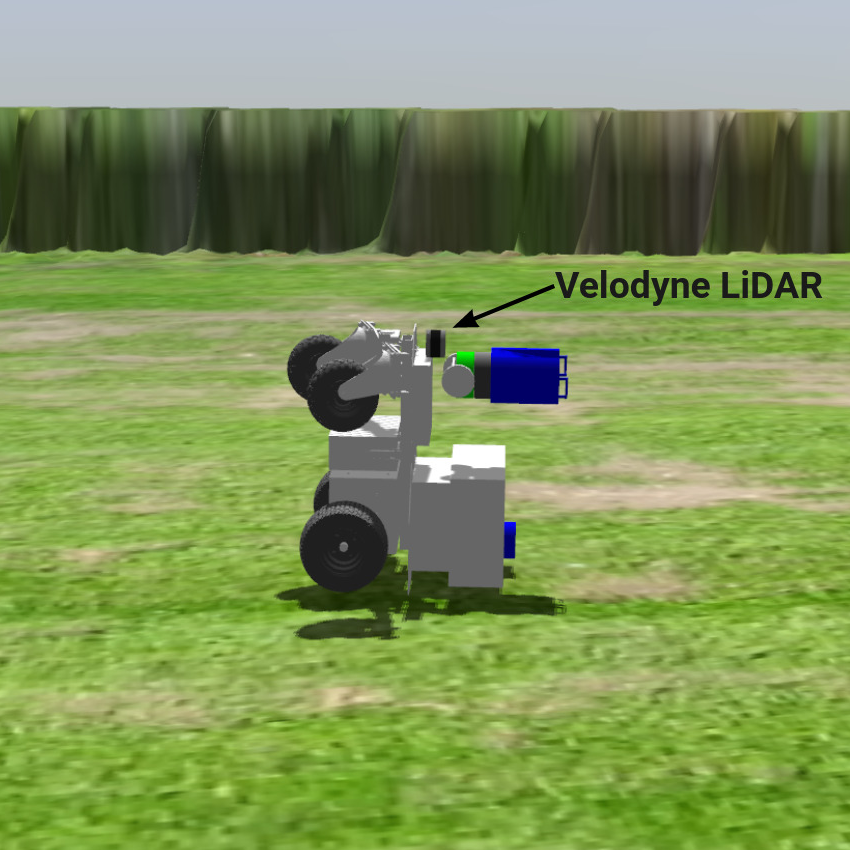
\includegraphics[width=0.8\textwidth]{pics/tilted_AROX.png}
        \caption{\textsc{Tilted AROX in Simulation}}
        \label{fig:tilted_AROX}
    \end{subfigure}
    \hfill
    \begin{subfigure}[b]{0.49\textwidth}
        \centering
        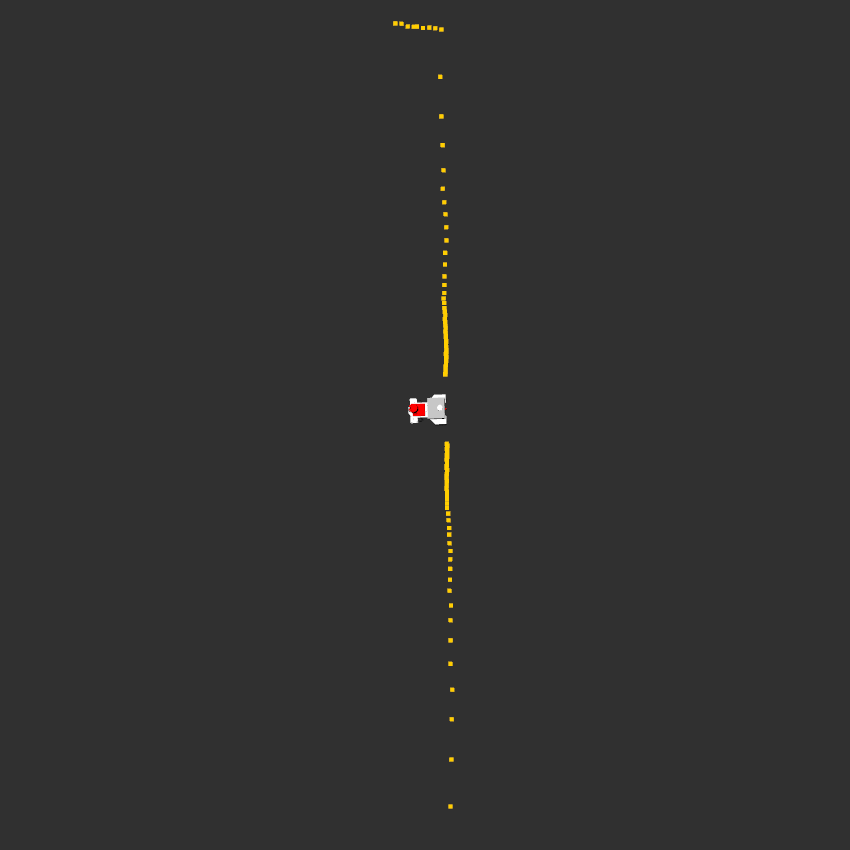
\includegraphics[width=0.8\textwidth]{pics/straight_line.png}
        \caption{\textsc{Feasible Range Values when Facing the Sky}}
        \label{fig:straight_line}
    \end{subfigure}
\caption{\textsc{Experiments with Tilted Sensor}}
\label{fig:prototype_sim}
\end{figure}
\noindent
The monitoring solution implements this approach by calculating the ratio between feasible and infeasible values and comparing it to the lower bound.
If the percentage of feasible range values does not exceed the lower bound, it is considered a sensor failure.
Moreover, it should be detected when no new scans arrive, i.e. the received scan is repeatedly the same.
To be able to compare the newly arrived scan with the previous one, the monitoring node always saves the last scan.
For the actual comparison, a unique hash value is calculated for both scans based on their range values as well as various metadata such as timestamp,
frame identifier, minimum and maximum angle, angle increment, time increment, scan time, and minimum and maximum range.
If the newly arrived scan has the same hash value as the previous one, such a sensor error has been detected.
In general, it is crucial to keep the monitoring solutions as general as possible, i.e. abstract from the specific sensors (\textit{RIEGL}, \textit{Velodyne})
in order to make them reusable for others. One hurdle standing in the way of this claim is the fact that many sensor manufacturers use their own proprietary data types.
Nevertheless, the underlying data is likely to be very similar. To provide some generality, the developed monitoring approaches will be able to handle the two data 
types commonly used in the ROS ecosystem, \code{LaserScan} and \code{PointCloud2}. In all cases, the sensor monitoring node publishes on the topic
\code{/contingency\_preemption} with a message that specifies the particular kind of sensor failure and causes a transition to the \code{CONTINGENCY} state.

\subsection{Data Management}
\label{sec:mon_data_management}

Similar to sensor (perception) monitoring, executing a \code{scan} action launches the data monitoring procedure, which looks for the potential data management issues presented in
section \ref{sec:challenges_for_lta}. To perform the drive capacity check, i.e. to determine whether the drive on which scan logging or data storage in general takes place has enough
free space, the cross-platform library \code{psutil}\footnote{https://pypi.org/project/psutil/} is used. It provides a function \code{disk\_usage()} which returns the load of the
specified disk, e.g. the one configured in \code{MONITOR\_DRIVE}. Unlike WiFi connection monitoring, where the actual low-level network connectivity checks are outsourced
from the monitoring framework due to its operating system coupling, disk capacity checks can be part of the framework itself because of the cross-platform nature of \code{psutil}.
If the result of \code{disk\_usage(MONITOR\_DRIVE)} exceeds $99\%$, the node detects a full memory and causes an interruption of the robot's mission and a transition to the
\code{CONTINGENCY} state. Additionally, notifications are sent to the operator when the disk load exceeds $95\%$ and $90\%$, with an indication that the data should be backed up
externally soon. So much for very general data management monitoring, which in principle can be used for all types of data acquisition tasks, since the type of data is irrelevant
to capacity testing. There is also a more scenario-specific part based on certain assumptions and dependencies that is optional and can be enabled or disabled by the user.
This is the specific scan logging monitoring that assumes that the data acquisition task at hand is a scanning task, such as the one described in section
\ref{sec:lta_plant_observation}, and that the scans are written to a user-configured directory in a file published by the dummy scanning node described in section
\ref{sec:dummy_scanning_node}. Since the data format of the scans written by the dummy scanner is well-known, i.e. \code{LaserScan} or \code{PointCloud2}, the entries logged in
this log file can be easily evaluated. The idea is that there should be an additional scan entry in the log file after a successful scan action. If that is not the case,
a data management error has been detected and a transition to \code{CONTINGENCY} is initiated. It would also be possible to implement some sort of exception escalation system
based on sensor logging errors, but since this would require in-depth knowledge of implementation details of the sensors used, it was renounced.\newline
General capacity monitoring is based on the idea of not having dependencies on specific scenarios or configurations, and instead just monitor the configured path and communicate
when certain thresholds are exceeded, which, as mentioned, basically works for any data acquisition task. However, the goal of ensuring a certain level of generality applies to
both cases. Of course, the second case is only suitable for laser scanning tasks, but it is not limited to one specific sensor. It can deal with all kinds of sensors that provide
results in the form of \code{LaserScan} or \code{PointCloud2}, which covers quite some generality. Therefore, a specific sensor such as the \textit{RIEGL} (cf. fig.
\ref{fig:arox_system}) can be replaced by another model without any problems, and data monitoring should continue to work based on the slight constraint of producing data of the
two mentioned types. General capacity monitoring works either way. Since the logging of the data always follows the scanning and the scanner is the module that writes the scans to
the file system, it would be superfluous to check the data again for plausibility, as this is already part of the sensor monitoring. It suffices to verify whether the storing
operation, i.e. writing the scan to the log file, worked. Moreover, it is worth noting that a total sensor failure always implies a data management failure of the second type,
but this should already be detected by the sensor monitoring procedure. Of course, more checks could be made for scenario-specific logs on the drive, etc., but since this would
require additional knowledge of the specific circumstances, it would violate the goal of being as general as possible. Nevertheless, it is possible to extend data management in
the future to include application-specific monitoring aspects that can be easily disabled to maintain general applicability.

\subsection{Lost Connection}
\label{sec:mon_lost_connections}

\subsubsection{WiFi Connection Failures}
\label{sec:mon_wifi_connection_problems}

Monitoring for WiFi connectivity problems takes place at two levels of abstraction. From the perspective of the high-level execution monitoring framework developed in this work,
the monitoring is completely independent of hardware and operating system details. However, monitoring the WiFi connection of a particular system depends heavily on such details,
so it is also necessary to provide low-level monitoring for network interfaces. The idea is that the high-level monitoring node expects the information that are evaluated as part 
of the monitoring in a very specific format on the ROS topic \code{/wifi\_connectivity\_info}. For this purpose, a custom ROS message \code{WiFi.msg} was defined consisting of the
three fields \code{float32 link\_quality}, \code{float32 signal\_level} and \code{float32 bit\_rate}. Therefore, it is irrelevant where this information comes from, it is simply
assumed to be provided. In order to demonstrate the WiFi monitoring in this work, the low-level operating-system-specific monitoring node that transfers this
information to the ROS system is implemented exemplarily for an Ubuntu system. It starts the Unix tool \code{iwconfig}
\footnote{https://manpages.debian.org/bullseye/wireless-tools/iwconfig.8.en.html} as a subprocess for a WiFi interface identifier that can be configured by the user. Subsequently,
the relevant information, i.e. link quality, signal level and bit rate, is parsed from the \code{iwconfig} output for the respective interface and a \code{WiFi.msg} is created
based on this. This message is then published under the \code{/wifi\_connectivity\_info} topic, which is subscribed by the high-level monitoring node. This process is repeated
continuously every $10$s.\newline
Now that it is clear how the low-level node works, the actual monitoring follows. As mentioned, the high-level monitoring node receives the WiFi information via the ROS topic
\code{/wifi\_connectivity\_info}. Based on this, the numerical information about the connection is evaluated. If all three provided values are $0$, it is considered
a disconnect and the monitoring solution induces a transition to the \code{CONTINGENCY} state. The link quality is evaluated based on three thresholds: If it is below $5\%$,
it is considered critically poor quality and a transition to \code{CONTINGENCY} follows. For the remaining two thresholds, the quality is not as bad as requiring a contingency
case, but it is still worth notifying the operator. For a link quality of $< 25\%$ a poor quality is reported, and for values less than $50\%$ a below average quality.
The signal level is also monitored based on three thresholds. As introduced in section \ref{sec:simulation_of_lta_challenges} it gets practically unusable for values below
$-90$ dBm. Thus, $\leq -90$ dBm acts as the trigger for a contingency case. Signal levels of $\leq -80$ dBm and $< -75$ dBm cause notifications of very weak and weak WiFi signals,
respectively. Finally, the bit rate is monitored based on two cases: if it is below $1$ Mb/s, a contingency is triggered, and if it is below $20$ Mb/s, a notification of a
rather low bit rate is transmitted. As soon as a malfunction is detected, monitoring is deactivated and resumed only when the problem has been solved. In all contingency
cases, the high-level WiFi monitoring node publishes on the topic \code{/contingency\_preemption} with a message that specifies the particular kind of connection problem.\newline
In summary, the problem of actually detecting the WiFi connectivity on the system in question is completely external to the execution monitoring framework,
which has no operating system coupling at all. There is a layer of abstraction that separates the two views. The assumption of the high-level monitoring framework is the
following: There is a node that publishes the WiFi connectivity for the system every $10$s int the \code{WiFi.msg} format. If someone wants to use the execution monitoring
framework on Windows, for example, there is no need to modify the framework's code, there just has to be an equivalent WiFi monitoring node for a Windows system that replaces
the Ubuntu-specific one.

\subsection{Obstacles Blocking the Planned Path}
\label{sec:mon_obstacles}

Recovery behaviors should naturally vary between static and dynamic obstacles. A dynamic obstacle like a person or an animal will in most cases 
simply walk through the scene and disappear a moment later, so waiting for a moment can already be a very reasonable and sufficient recovery behavior. 
Static obstacles, on the other hand, may be present for longer  periods of time, requiring more sophisticated recovery behaviors.

\subsection{Navigation Failure}
\label{sec:mon_navigation_failures}

To overcome the problems, one could develop specific recovery behaviors for the considered scenario, analogous to Duchetto et al.

\subsection{Sustained Recovery}
\label{sec:mon_sustained_recovery}

In this case, the robot should try a few different recovery actions and then abort and report the problem.
Monitoring methods must therefore track the results of recovery behaviors and decide whether it is appropriate to try more or stop.

\subsection{Incorrect or Inaccurate Localization}
\label{sec:mon_incorrect_localization}

It would be very valuable to develop a monitoring approach that is capable of realizing situations in which the localization is no longer accurate, as there is a 
simple workaround that alleviates the problem in practice in many cases: Just driving the robot a few meters back and forth to recalibrate the localization
using different GNSS positions. Since the localization is based not only on GNSS, but also on IMU and odometry data, it would also be very valuable to identify
the errors that occur there, but that is beyond the scope of this work.

\subsection{Plan Deployment Failure}
\label{sec:mon_plan_deployment_failures}

A first solution attempt that the robot should definitely try would be to retrigger the plan generation service described in section \ref{sec:plan_generation}. 
If this does not help, it should waste no time and immediately notify the operator.

\section{Solutions for LTA Challenges}
\label{sec:solutions_for_lta_challenges}

As anticipated, the focus of the work is on detection, and an initial solution adopted for all the issues identified in section \ref{sec:challenges_for_lta} will be 
to communicate the problem to a human operator. Requesting the help of the human operator not only serves as an initial solution, but is always acting as fallback 
solution when other solution attempts are unsuccessful. The idea is to have the monitoring procedures described in section \ref{sec:monitoring_for_lta_challenges} that 
look for the specific types of issues and initiate an appropriate response.\newline
Whenever a monitoring solution described in section \ref{sec:monitoring_for_lta_challenges} causes a transition to the \code{CONTINGENCY} or \code{CATASTROPHE} states
by publishing on the respective topics \code{contigency\_preemption} or \code{catastrophe\_preemption}, information about the cause of the interruption is
transmitted via a ROS message. Based on this cause, the corresponding resolver class is selected and executed. The idea is that each general problem class, e.g.
connection problems, provides a resolution method for each potential specific problem in that class, e.g. poor WiFi link quality. The \code{CONTINGENCY} state in turn
communicates the failure reason to the resolver classes. If available, the specific resolving method will be executed. Afterwards, the outcome is reported back to the
high-level state machine, which either continues normal operation if the problem is successfully solved, or aggravates to catastrophe, for example. If the specific resolver
method is not able to handle the problem, or if there is not even a specific resolver method for the failure case, the problem is handed over to the fallback resolver,
which passes the problem to the human operator and awaits resolution. If the respective failure was caused by a simulation, the corresponding flag must be reset to restore
normal operation, which is done by publishing on the particular toggle topic described in section \ref{sec:simulation_of_lta_challenges}.\newline

\noindent
\textbf{Communication with a Human Operator}\newline

\noindent
Communication with a human operator, i.e. notifying a human operator that a problem has occurred that requires human intervention or providing useful information about the state
of the robot or mission, is implemented as a separate \code{OperatorCommunication} class. The robot-human communication module is subscribed to three different topics. First,
a message on \code{/request\_help\_contingency} indicates that the robot is requesting the help of a human operator, but is still functioning in principle. The second topic
\code{/request\_help\_catastrophe} is used for more severe cases where the robot needs human help and is inoperable, e.g. has a full breakdown. Finally, there is \code{/robot\_info},
which is used for minor problems or tasks that do not require immediate action, but are good to know and tackle soon, e.g. a memory usage of $90\%$. In the first two cases, control
can be returned to the autonomous mobile robot via the \code{/problem\_solved} topic once the problem has been solved by the human operator. All the monitoring modules described
in section \ref{sec:monitoring_for_lta_challenges} are subscribed to the \code{/robot\_info} topic and thus able to communicate relevant information. The more critical topics for
contingency and catastrophe cases can be triggered by the fallback resolver described in the last section.

\chapter{Integrated Solutions}

In general, an integrative work benefits from many integrated solutions. Nevertheless, it should be viable in the scope of the work and robust.
Essentially, there is a tradeoff between integrating as much as possible, thereby increasing the functionality, and staying feasible and realistic.
The following subsections present exemplary approaches that may be integrated. The list could be expanded as needed during the course of the work.

\section{Battery Monitoring}
\label{sec:battery_monitoring}

One solution that could be worth integrating is a watchdog module that observes the battery state and acts as a fail-safe. In principle, the charge stops should
be part of the plan, i.e. be considered at planning time. Thus, there has to be resource planning for the missions that includes to be back at the base station before
the robot runs out of battery. However, if it fails, there could be a monitoring process at execution time that is able to react to wrong plans, i.e. the battery is
low before expected and the robot has to return to its base. The module essentially checks the distance from the robot's current position to the base station, 
the expected battery consumption to get there, and the remaining battery charge. In summary, the module is running at execution time, it does not schedule the 
charge stops in advance, but only responds to failure cases where the robot needs to preempt the plan execution, return to its base and recharge.
Such a battery watchdog is an example for monitoring tools relevant for addressing the challenges introduced in section \ref{sec:challenges_for_lta}.

\section{Autonomous Energy Supply}
\label{sec:docking_solution}

A fundamental step towards long-term autonomy of a mobile robot is to ensure its power supply.
For this purpose, there is an inductive charging station located in a mobile container on the field site.
Thus, the power supply could be realized by integrating an autonomous docking / undocking solution that enables the robot to detect
the container in a laser scan of its nearby surroundings, drive into it and dock to the inductive charging station.
This docking solution could be used for both planned charge stops as well as unexpected but necessary stops detected by monitoring processes such
as the one described in section \ref{sec:battery_monitoring}.

\bibliography{papers}

\begin{appendices}
    \chapter{Detailed Results of Questionnaire}
    \label{sec:detailed_questionnaire_results}

    \begin{figure}[H]
        \centering
        \resizebox{0.75\textwidth}{!}{
        \begin{tabular}{| c | c | c | c | c |}
            \hline
            \textbf{problem} & \textbf{impact} & \textbf{difficulty} & \textbf{likelihood} \\ \hline
            charging\_failure & [1, 2, 1, 1, 2, 1, 1] & [1, 2, 1, 2, 1, 1, 1] & [2, 2, 2, 1, 3, 1, 1] \\ \hline
            incorrect\_localization & [2, 1, 1, 2, 1, 2, 2] & [2, 3, 2, 2, 3, 2, 2] & [2, 2, 2, 1, 1, 2, 1] \\ \hline
            power\_management & [1, 1, 1, 1, 1, 1, 1] & [1, 1, 1, 3, 1, 2, 1] & [2, 3, 2, 1, 2, 2, 2] \\ \hline
            data\_management & [1, 2, 2, 2, 2, 1, 1] & [2, 2, 3, 1, 2, 2, 2] & [1, 2, 2, 2, 2, 2, 2] \\ \hline
            sustained\_recovery & [1, 2, 1, 2, 1, 1] & [2, 2, 2, 3, 3, 3] & [2, 2, 1, 2, 3, 2] \\ \hline
            mapping\_error & [2, 2, 1, 2, 2, 2, 2] & [2, 3, 1, 2, 3, 2, 2] & [2, 2, 2, 1, 1, 2, 2] \\ \hline
            navigation\_failure & [1, 1, 3, 2, 2, 2, 2] & [2, 1, 2, 3, 2, 2] & [2, 3, 1, 1, 2, 2] \\ \hline
            robot\_gets\_stuck & [1, 1, 2, 1, 3, 1, 1] & [2, 3, 3, 1, 3, 2, 2] & [3, 2, 3, 2, 1, 2, 2] \\ \hline
            sensor\_failure & [1, 1, 2, 1, 2, 2, 2] & [1, 1, 2, 2, 2, 2, 2] & [1, 3, 2, 3, 2, 2, 2] \\ \hline
            lost\_connection & [2, 1, 2, 3, 3, 2, 2] & [1, 1, 3, 1, 2, 2, 3] & [2, 1, 3, 1, 1, 1, 2] \\ \hline
            plan\_deployment\_failure & [1, 2, 1, 2, 2, 2] & [2, 1, 2, 2, 2, 2] & [2, 3, 1, 2, 3, 2] \\ \hline
            obstacles\_blocking\_path & [2, 3, 2, 2, 2, 2, 3] & [2, 3, 3, 1, 2, 2, 2] & [2, 1, 3, 1, 1, 1, 1] \\ \hline
            drastic\_weather\_change & [2, 2, 1, 2, 2, 2, 2] & [2, 3, 2, 3, 3, 2, 2] & [3, 2, 2, 2, 3, 2, 2] \\ \hline
            certain\_dynamics & [2, 3, 3, 2, 2, 2, 3] & [2, 1, 1, 3, 1, 1, 1] & [2, 3, 1, 1, 3, 1, 1] \\ \hline
            robot\_falls\_over & [1, 1, 1, 1, 1, 1, 1] & [3, 2, 1, 2, 3, 3] & [3, 3, 2, 3, 2, 3] \\ \hline
            perceptual\_aliasing\_issue & [2, 2, 1, 2, 3, 2] & [2, 2, 3, 3, 3, 2] & [2, 2, 3, 2, 3, 2] \\ \hline
        \end{tabular}}
    \caption{\textsc{Results of the Questionnaire (cf. section \ref{sec:relevance_assessment})}}
    \label{fig:average_results_2d}
    \end{figure}
\end{appendices}

\closing %%%%%%%%%%%%%%%%%%%%%%%%%%%%%%

\end{document}
